\documentclass[10pt]{article}
\usepackage[margin=1in]{geometry}
\usepackage[utf8]{inputenc}
\usepackage[T1]{fontenc}
\usepackage{microtype}
\usepackage{amsmath,amssymb}
\usepackage{mathtools}
\usepackage{graphicx}
\graphicspath{{figures/}}
\usepackage{booktabs}
\usepackage[round]{natbib}
\usepackage{hyperref}
\usepackage{xcolor}
\usepackage{caption}
\usepackage{subcaption}
\usepackage{enumitem}
\usepackage{wrapfig}

\setlength{\parskip}{0.4em}
\setlength{\parindent}{0em}

\title{\textbf{A Benchmark and an Open Problem:\\Fractal-Basin Classification for the Planar Three-Body Problem}}

\author{
  Aishwarya Das\\
  Dirac Labs Inc.\\
  \texttt{aishwarya@diraclabs.com}
}

\date{}

\begin{document}
\maketitle

% ============================================================================
\begin{abstract}
The escape basins of the gravitational three-body problem have fractal boundaries whose geometry constrains learnability. We release a benchmark of $10^6$ labeled initial conditions on the Montgomery shape sphere (2D, at rest) and $10^6$ in the reduced 6D phase space, with per-trajectory integration diagnostics and Wada topology characterization. Boundary-targeted active learning improves classifier macro-F1 by $+3.7\%$ in 2D but degrades it by $-0.7\%$ in 6D, where the uncertainty dimension $D_u = 5.86$ causes the fractal boundary to nearly fill the phase space. Under architecture-specific training, measured error-scaling slopes are consistent with the 1983 Grebogi-Ott-Yorke prediction to 6--9\% for two architectures. Under a pre-registered matched-compute protocol, slopes are flat; training diagnostics reveal differential convergence as the root cause. Whether classifier scaling tightly matches the GOY bound under properly matched training remains an open question. We release all data and code.
\end{abstract}

% ============================================================================
\section{Introduction}

The gravitational three-body problem is a canonical example of deterministic chaos: the long-term trajectory of three interacting masses is generically unpredictable, yet the asymptotic outcome, which body escapes from the remaining binary, is a well-defined classification problem. The decision boundaries of this classification are the \emph{basin boundaries} of the dynamical system, which are known to be fractal in chaotic scattering systems \citep{GOY1983, MGOY1985}.

\begin{figure}[t]
  \centering
  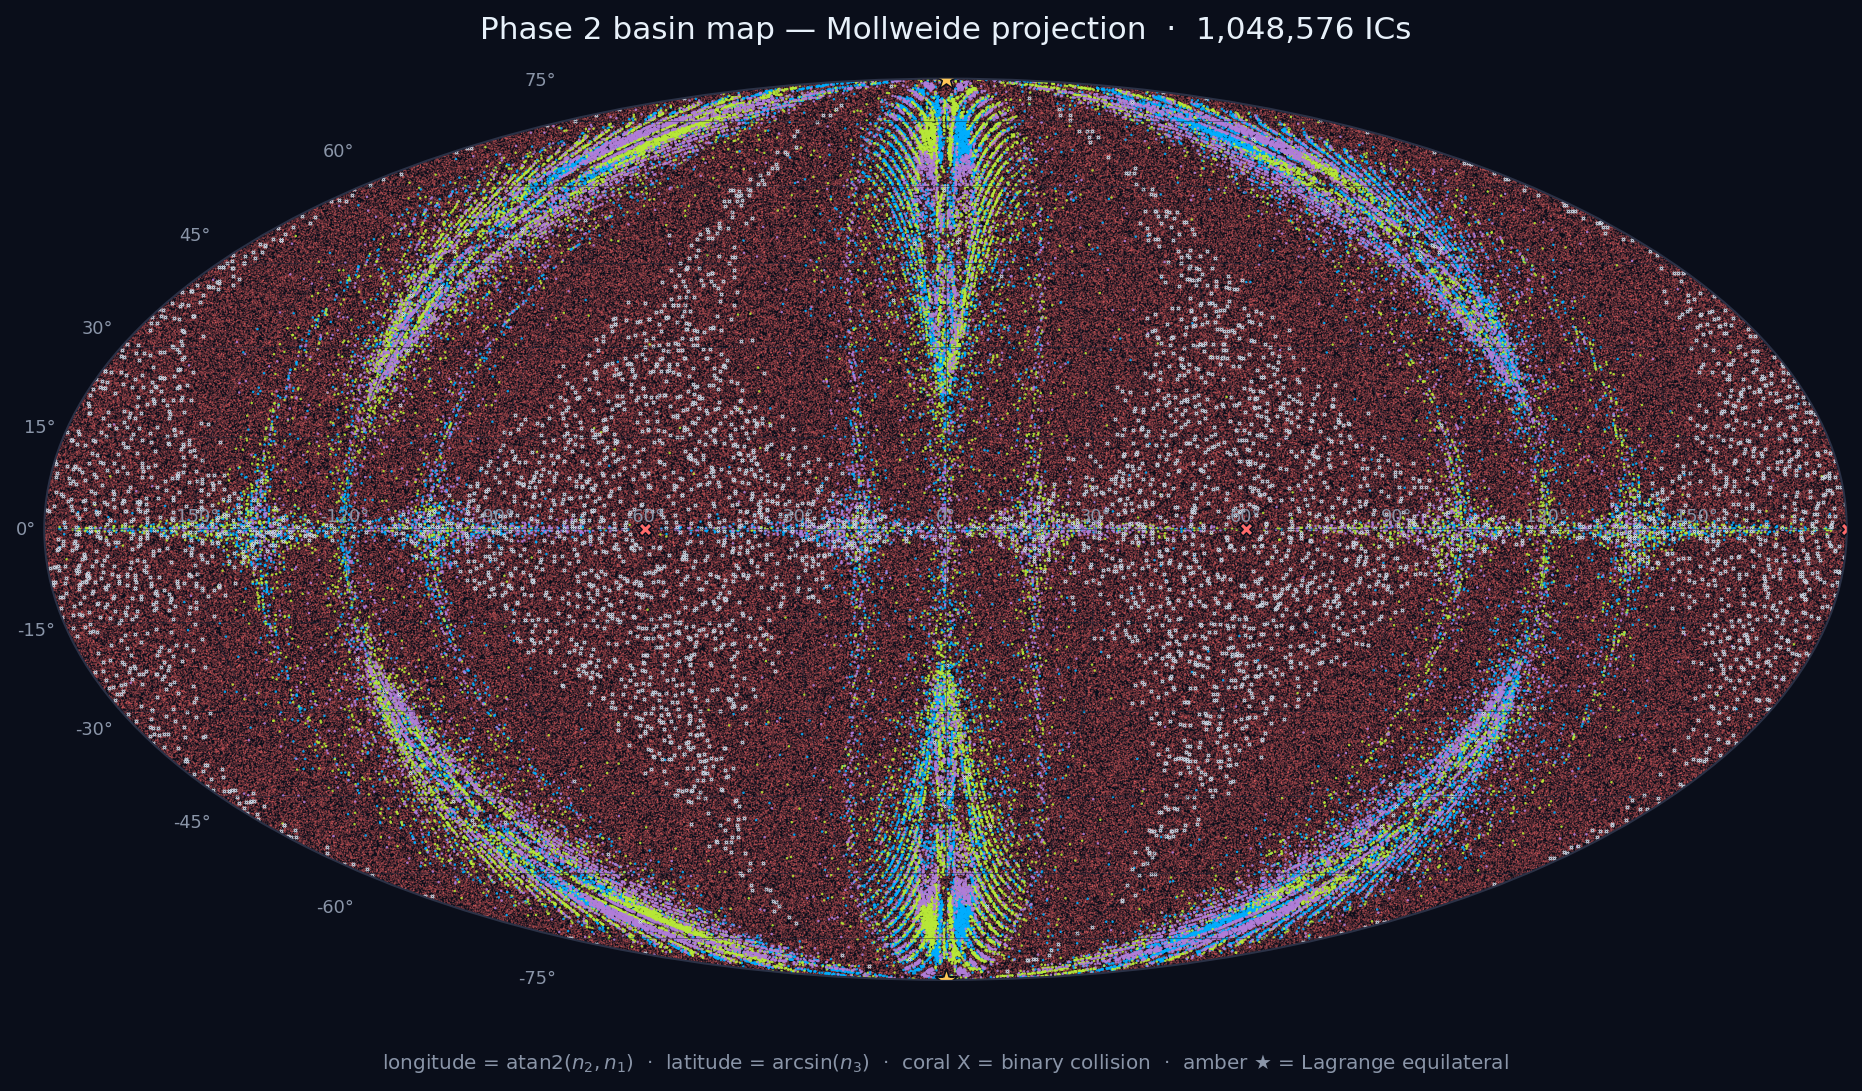
\includegraphics[width=\linewidth]{basin_mollweide.png}
  \caption{Escape basins of the equal-mass planar three-body problem on the Montgomery shape sphere (Mollweide projection, ${\sim}10^6$ initial conditions at rest). Four outcome classes are shown: bound orbits and three single-body escape channels. The $120^\circ$ rotational symmetry of the $S_3$ permutation group is visible. Basin boundaries are fractal and satisfy the Wada property: every boundary point simultaneously borders all three escape basins.}
  \label{fig:basins}
\end{figure}

A classical result of \citet{GOY1983} connects fractal geometry to predictability: for a classifier trained on $N$ uniformly sampled points in $d$ dimensions, the test error scales as $\text{error}(N) \sim N^{-\alpha/d}$, where $\alpha$ is the \emph{uncertainty exponent} measuring how quickly the fraction of ambiguous initial conditions vanishes with perturbation magnitude. This bound has been a theoretical fixture for four decades, but no quantitative test has been performed on a physically grounded system using modern neural classifiers.

We contribute three things. First, a reproducible benchmark dataset on the Montgomery shape sphere \citep{Montgomery2015} (2D, $10^6$ initial conditions; Figure~\ref{fig:basins}) and in the full 6D reduced phase space ($10^6$ initial conditions with non-zero momenta), with per-trajectory integration diagnostics. Second, a clean empirical finding: active learning that targets basin boundaries helps in 2D but fails in 6D, explained by the uncertainty dimension. Third, an open methodological problem: classifier error-scaling slopes match the GOY prediction under architecture-specific training but not under matched-compute training, with a mechanistic diagnostic explaining why.

% ============================================================================
\section{Related Work}

\citet{Trani2024} mapped the escape-basin structure of the three-body problem across a 2D parameter slice and measured multi-fractal correlation dimensions $D_2 \approx 1.65$--$2.0$. \citet{UmeharaTanikawa1998} studied binary and triple collisions in the free-fall three-body problem. The fractal-basin framework originates with \citet{GOY1983} and \citet{MGOY1985}, who introduced the uncertainty exponent and its measurement protocol. \citet{NusseYorke1992} and \citet{Poon1996} established the Wada property for multi-basin chaotic scattering. \citet{Aguirre2001} studied Wada basins in the H\'enon-Heiles system. \citet{Daza2016} introduced basin entropy as a complementary diagnostic, and \citet{Daza2018} developed the merging test for the Wada property.

Neural classifiers for basin prediction have been explored by \citet{Shena2021} and \citet{Valle2024} on low-dimensional dynamical systems. Machine learning for the three-body problem specifically has focused on trajectory prediction \citep{Breen2020, Liao2022} rather than basin classification. Statistical escape theories \citep{StoneLeigh2019, Manwadkar2021, Kol2021} provide complementary analytical frameworks. Our $S_3$-equivariant architecture draws on the DeepSets framework \citep{DeepSets2017}.

% ============================================================================
\section{Benchmark and Setup}

\begin{figure}[t]
  \centering
  \begin{minipage}[t]{0.42\linewidth}
    \centering
    
\includegraphics[width=\linewidth]{shape_sphere_3d.png}
    \captionof{figure}{The Montgomery shape sphere $S^2$ parameterizing three-body configurations modulo translation, rotation, and scaling. Binary-collision singularities $C_{12}$, $C_{13}$, $C_{23}$ lie on the equator at $120^\circ$ intervals. Lagrange equilateral configurations $L_+$, $L_-$ occupy the poles.}
    \label{fig:shape_sphere}
  \end{minipage}\hfill
  \begin{minipage}[t]{0.55\linewidth}
    \centering
    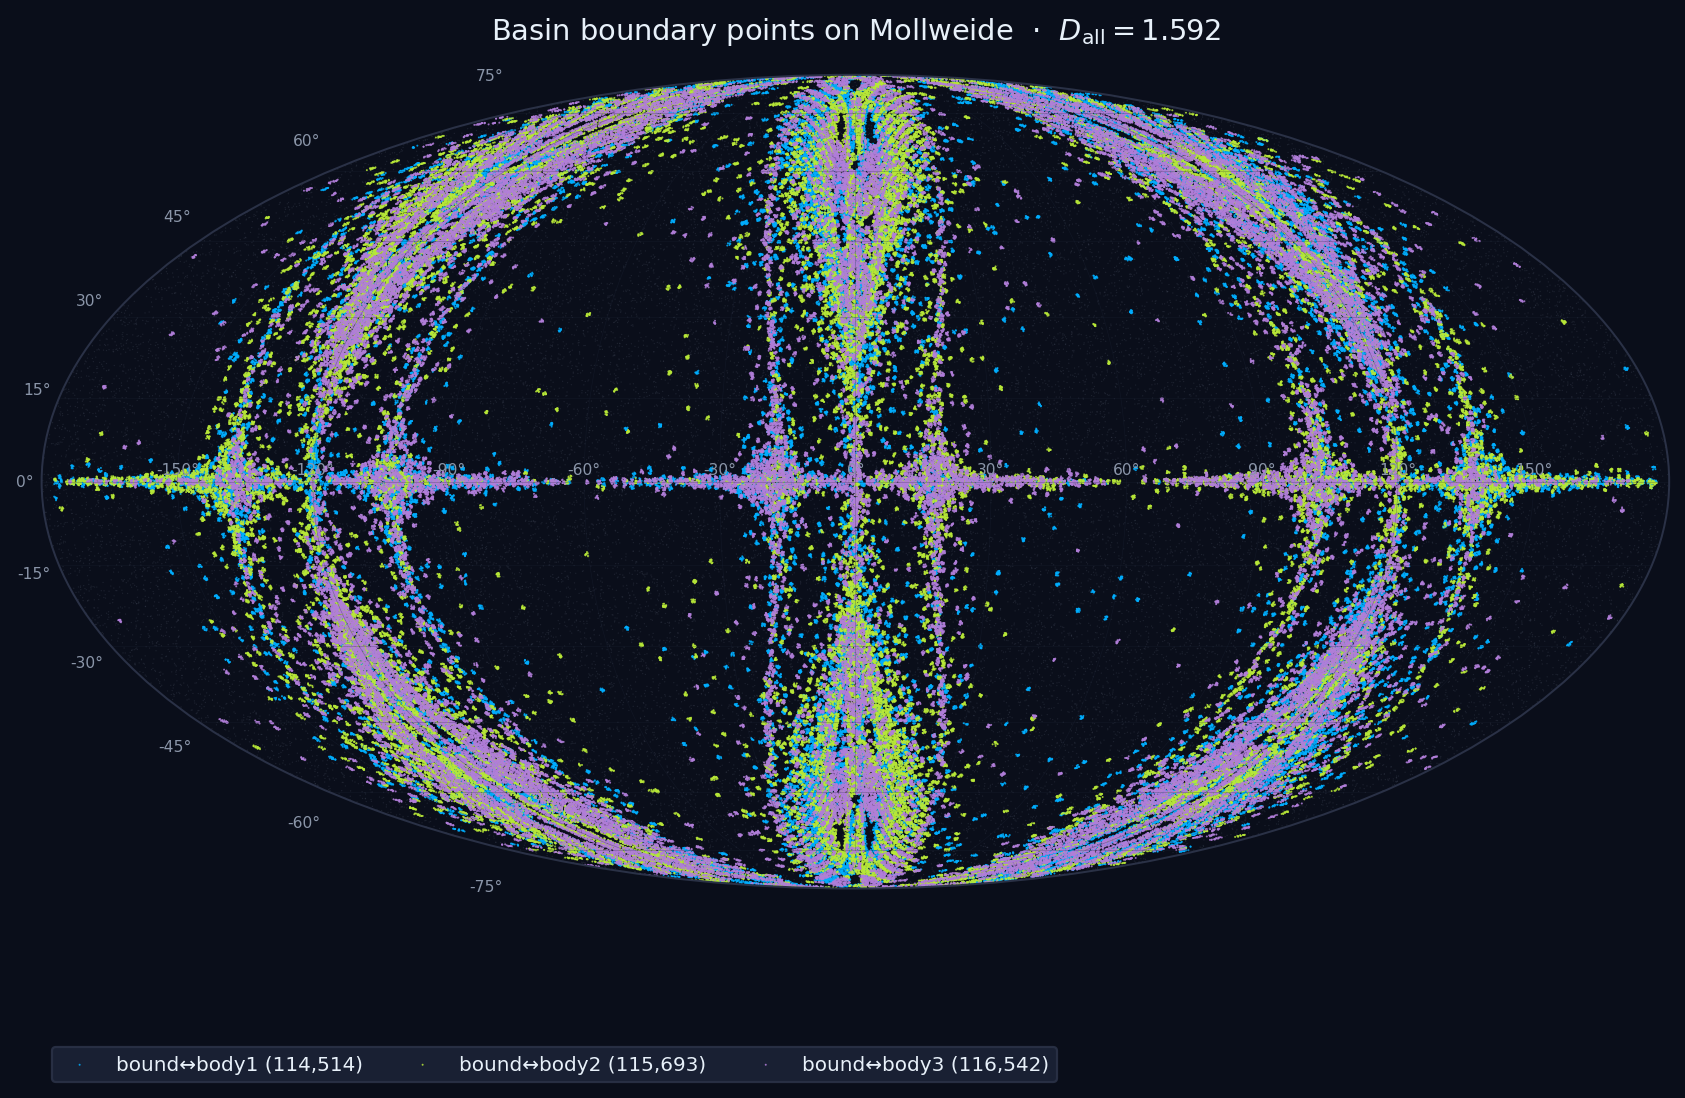
\includegraphics[width=\linewidth]{fractal_mollweide.png}
    \captionof{figure}{Basin boundary points (Mollweide projection). Points whose nearest neighbor in perturbation space has a different class label are plotted, revealing the fractal geometry. The three colors correspond to three boundary pairs; all three overlap everywhere, confirming the Wada property. Box-counting dimension $D_{\text{all}} = 1.59$.}
    \label{fig:fractal}
  \end{minipage}
\end{figure}

\textbf{Shape sphere.}\quad The configuration space of three equal-mass bodies in the plane, modulo translation, rotation, and scaling, is the Montgomery shape sphere $S^2$ \citep{Montgomery2015} (Figure~\ref{fig:shape_sphere}). A point on this sphere is parameterized by coordinates $(n_1, n_2, n_3)$ with $n_1^2 + n_2^2 + n_3^2 = 1$. Three binary-collision singularities sit $120^\circ$ apart on the equator; the Lagrange equilateral configurations occupy the poles.

\textbf{Integration.}\quad We integrate the Newtonian equations of motion using a 6th-order Yoshida symplectic integrator \citep{Yoshida1990} with adaptive timestep. Trajectories that approach a close encounter below $r_{\min} = 0.01$ length units at any point during integration are excluded, removing 9.1\% of the 2D sample and 3.4\% of the 6D sample. We classify each surviving trajectory by the Standish escape criterion: a body is considered escaped when it reaches hyperbolic velocity relative to the remaining binary.

\textbf{Datasets.}\quad The 2D at-rest dataset contains $953{,}143$ clean labeled trajectories (after close-encounter exclusion) uniformly sampled on $S^2$ with zero initial momenta. The 6D dataset contains $1{,}010{,}567$ clean trajectories with non-zero Jacobi momenta sampled uniformly in the reduced phase space. Both are four-class problems: bound (no escape within the integration window) and three escape outcomes (body 1, 2, or 3). The 2D dataset is approximately 94\% bound.

\textbf{Uncertainty exponent.}\quad We measure $\alpha$ via the MGOY algorithm \citep{MGOY1985}: for each perturbation scale $\varepsilon$, we sample $10^5$ pairs of initial conditions separated by $\varepsilon$ and compute the disagreement fraction $f(\varepsilon)$. A power-law fit $f(\varepsilon) \sim \varepsilon^\alpha$ yields $\alpha_{2D} = 0.259 \pm 0.019$ ($R^2 > 0.999$) and $\alpha_{6D} = 0.145 \pm 0.004$ ($R^2 = 0.999$). The corresponding uncertainty dimensions are $D_u^{2D} = d - \alpha = 1.74$ and $D_u^{6D} = 5.86$.

\textbf{Wada topology.}\quad We apply the merging test of \citet{Daza2018} to the 2D basins (Figure~\ref{fig:fractal}): iteratively merging pairs of basin classes and checking whether the basin boundary remains unchanged. All three escape basins share a common boundary, confirming the Wada property. The basin entropy is $S_b = 0.222$ and the basin boundary entropy is $S_{bb} = 0.472$ \citep{Daza2016}.

% ============================================================================
\section{Active Learning in 2D vs 6D}

Does boundary-targeted sampling help on fractal-basin classification? We compare two acquisition strategies at matched total labeling budget: \emph{uniform} sampling (i.i.d.\ from the domain) and \emph{active learning} using $k$-nearest-neighbor disagreement detection with tangent-plane perturbation (perturbation scale $\sigma = 0.005$ rad in 2D). At each acquisition round, the AL strategy selects points near detected class boundaries; the uniform strategy draws points at random.

\begin{figure}[t]
  \centering
  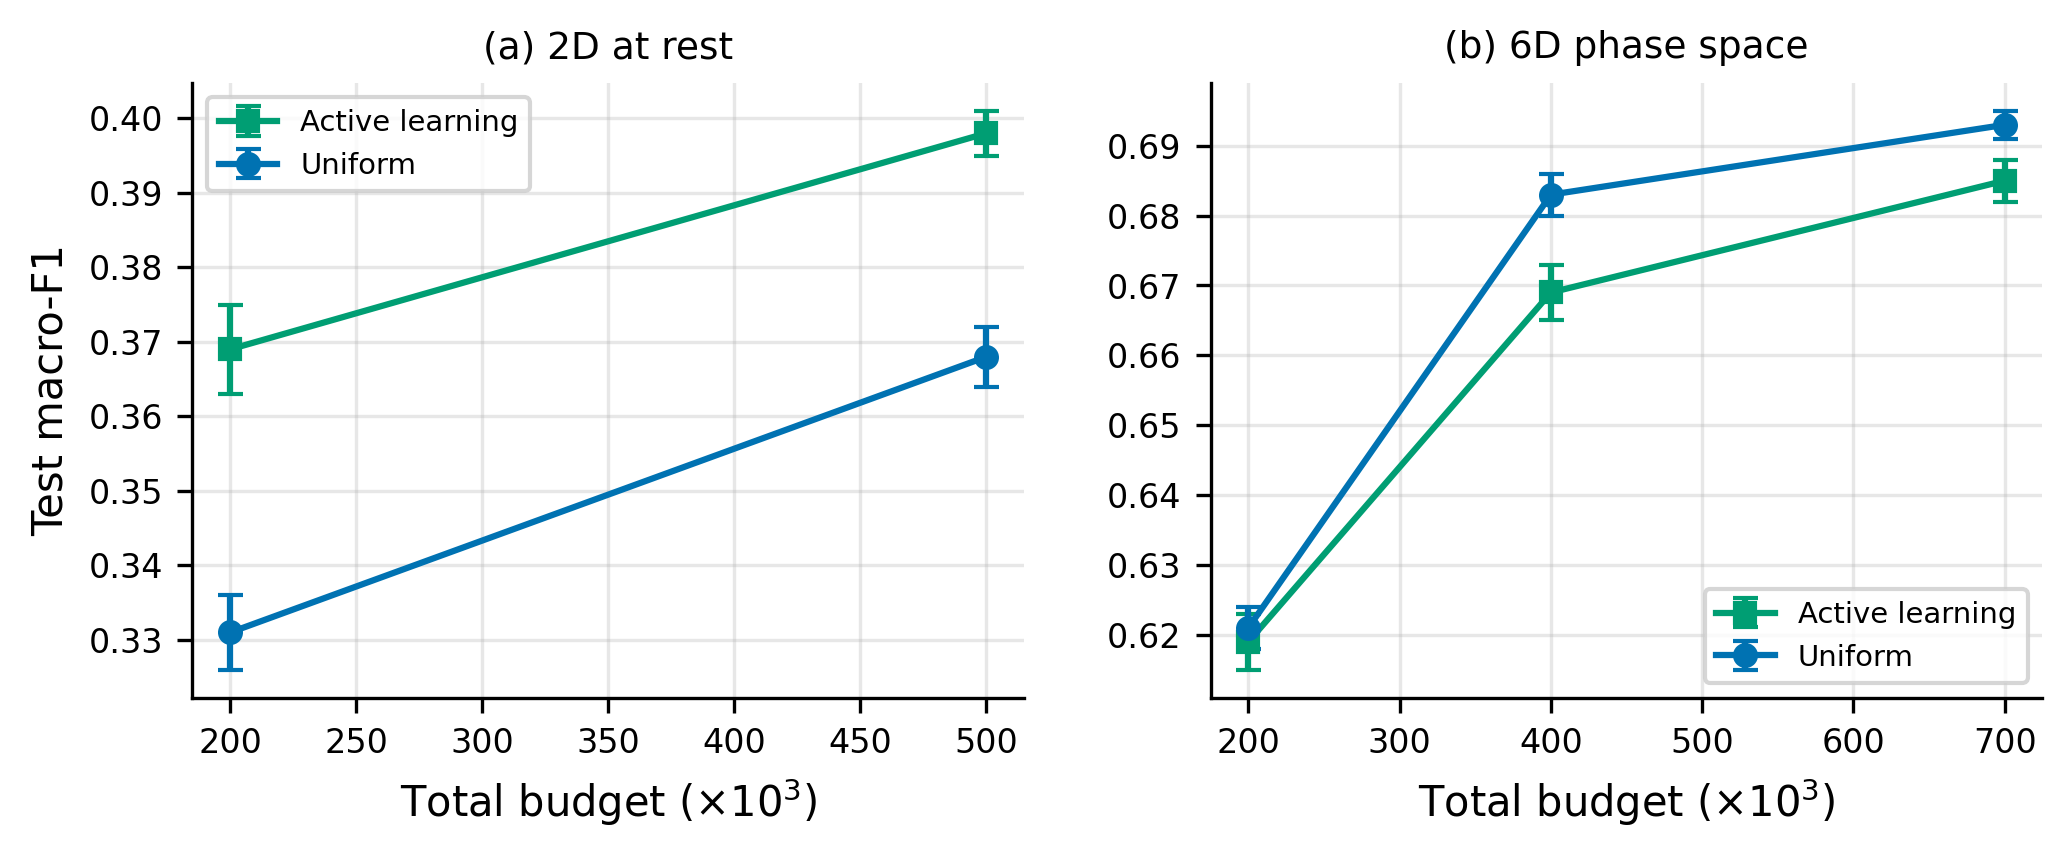
\includegraphics[width=\linewidth]{F2_al_2d_6d.png}
  \caption{Active learning versus uniform sampling at matched labeling budget. (a) In 2D, AL consistently outperforms uniform sampling, with the gap widening at larger budgets. (b) In 6D, uniform sampling performs as well or better than AL at every budget tested. Error bars are $2\sigma$ over 5 seeds. The reversal is explained by the uncertainty dimension: $D_u = 1.74$ in 2D (boundary is localized) versus $D_u = 5.86$ in 6D (boundary nearly fills the space).}
  \label{fig:al}
\end{figure}

Figure~\ref{fig:al} shows the results. In 2D, active learning improves macro-F1 by $+3.7\%$ at budget $B = 500$k (from $0.368$ to $0.398$). In 6D, uniform sampling outperforms active learning at every budget tested, with AL degrading macro-F1 by $-0.5\%$ to $-1.0\%$.

The explanation lies in the uncertainty dimension. In 2D, $D_u = 1.74$: the basin boundary is a fractal curve of dimension $1.74$ embedded in a 2D space, occupying a vanishing fraction of the domain at finite resolution. Boundary-targeted sampling concentrates labels where they are most informative. In 6D, $D_u = 5.86$: the boundary nearly fills the 6-dimensional phase space. At any practical resolution, a randomly chosen point is already near a class boundary, so ``targeted'' sampling degenerates into a noisy approximation of uniform sampling, with the added overhead of $k$-NN queries. The implication for practitioners is direct: active learning heuristics premised on localized uncertainty fail when uncertainty is spatially uniform, as occurs in high-dimensional fractal-basin systems.

% ============================================================================
\section{The Scaling-Law Question}

The GOY bound \citep{GOY1983} predicts that classifier test error on fractal basins scales as $\text{error}(N) \sim N^{-\alpha/d}$. For our 2D dataset with $\alpha = 0.259$ and $d = 2$, the predicted log-log slope is $-\alpha/d = -0.130 \pm 0.010$.

\subsection{Architecture-specific training}

We train two architectures across $N \in \{10\text{k}, 30\text{k}, 100\text{k}, 300\text{k}\}$ with 5 seeds each. The \textbf{MLP} is a 6-layer feed-forward network with 384 hidden units, taking 3D shape-sphere coordinates as input, trained for 60 epochs with cosine learning-rate annealing. \textbf{S3BodyNet} is a permutation-equivariant architecture \citep{DeepSets2017} with shared per-body feature extraction and symmetric pooling, taking 7D input (shape-sphere coordinates plus zero-padded Jacobi momenta), trained for 200 epochs under the same optimizer.

Figure~\ref{fig:scaling}a shows the results. The MLP produces a slope of $-0.131 \pm 0.005$, and S3BodyNet produces $-0.141 \pm 0.009$. Under architecture-specific training, measured slopes are consistent with the GOY prediction to 6--9\%.

\begin{figure}[t]
  \centering
  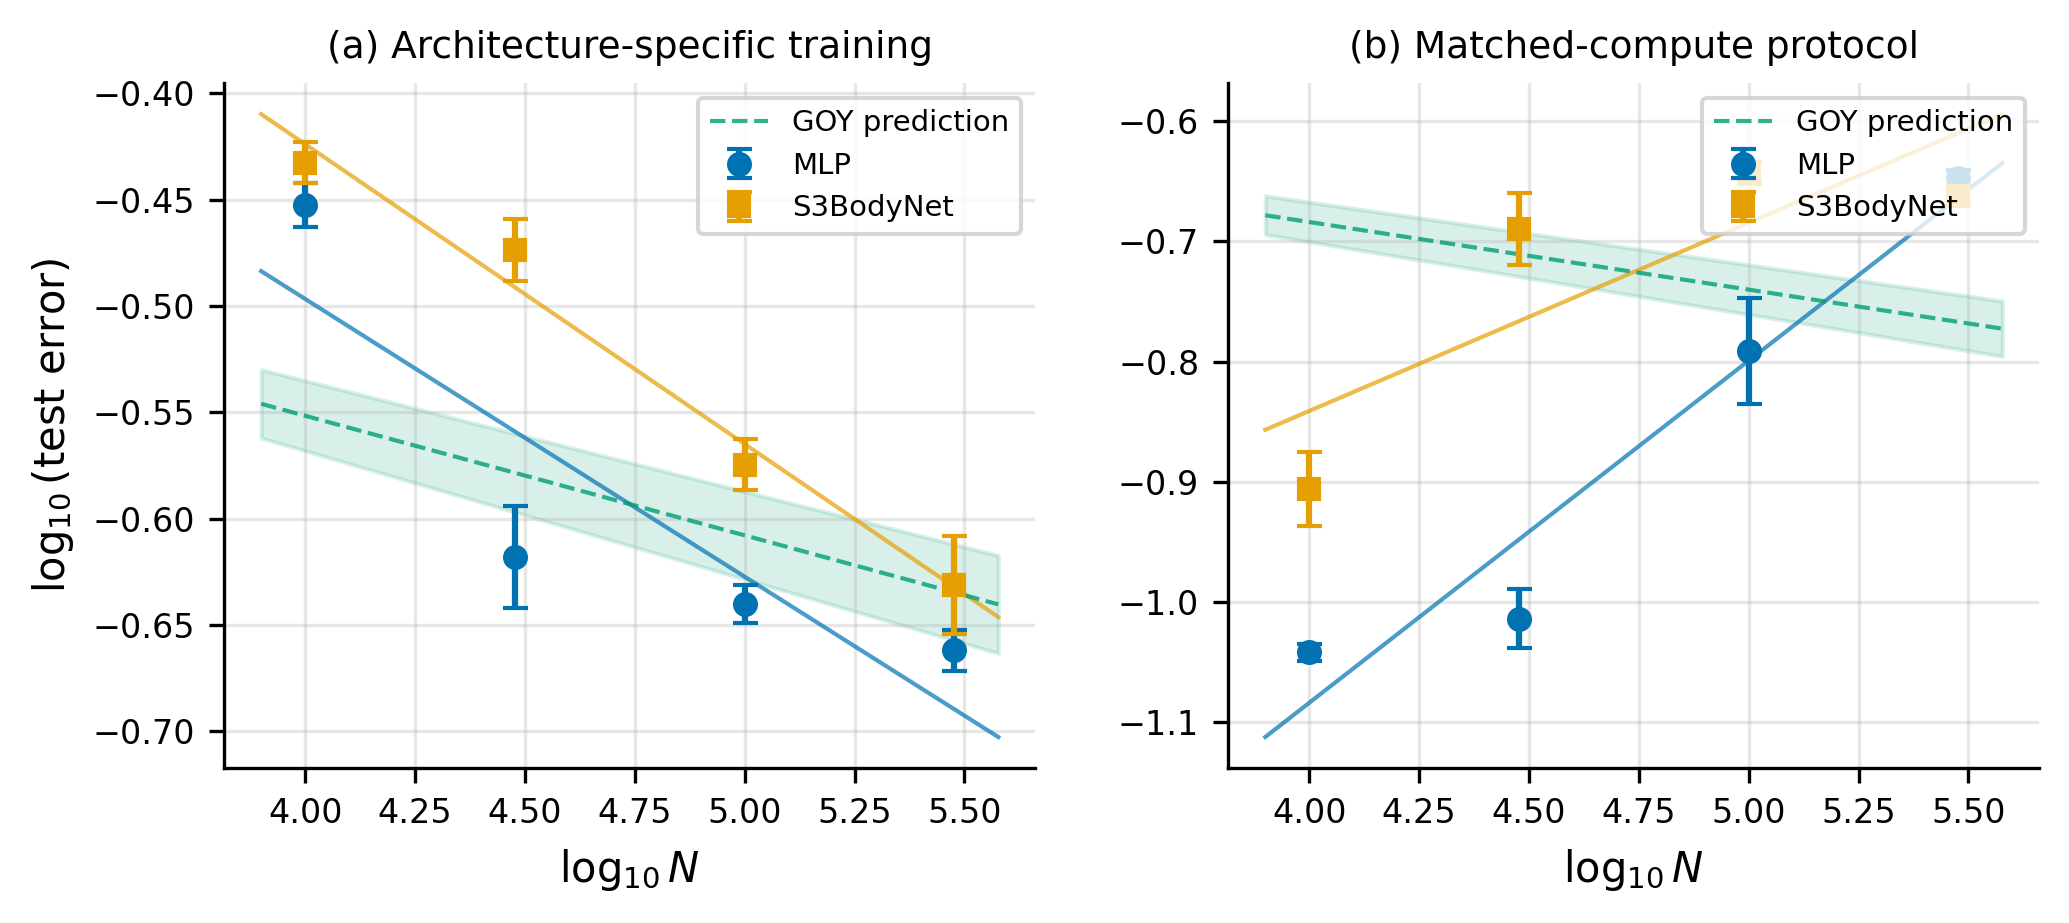
\includegraphics[width=\linewidth]{F3_scaling_law.png}
  \caption{Test error versus training set size on a log-log scale. Green band shows the GOY prediction $\pm 2\sigma$. (a)~Under architecture-specific training (MLP at 60 epochs, S3BodyNet at 200 epochs), both slopes fall within the GOY band. (b)~Under a matched-compute protocol (identical optimizer, learning rate, and gradient-update budget for both architectures), slopes are flat or inverted, far from the GOY prediction. The contrast between the two panels is the central finding of this paper.}
  \label{fig:scaling}
\end{figure}

\subsection{Matched-compute protocol}

The architecture-specific result confounds training schedule with architecture. An MLP trained for 60 epochs and an S3BodyNet trained for 200 epochs receive different numbers of gradient updates, different learning-rate trajectories, and different convergence characteristics. To isolate the scaling law from training choices, we ran a pre-registered matched-compute test.

The protocol fixes all training hyperparameters across architectures: AdamW optimizer, batch size 1024, a single learning rate (tuned once per architecture on a held-out validation slice), 500-step linear warmup, cosine decay to zero, and a fixed budget of 58{,}594 gradient updates per cell (equivalent to 200 epochs at $N = 300$k). No early stopping. Five seeds $\{0, 1, 2, 3, 4\}$. Four dataset sizes $N \in \{10\text{k}, 30\text{k}, 100\text{k}, 300\text{k}\}$. Pre-registered pass criterion: both slopes within $2\sigma$ of the GOY prediction and within $2\sigma$ of each other.

Figure~\ref{fig:scaling}b shows the results. The MLP slope is $-0.002 \pm 0.003$ ($R^2 = 0.01$), and the S3BodyNet slope is $+0.014 \pm 0.002$ ($R^2 = 0.51$). Both are far from the GOY prediction. The test failed all three agreement criteria.

\subsection{Why the disagreement}

The fixed gradient-update budget creates a fundamental asymmetry across dataset sizes. At $N = 10$k, 58{,}594 updates means approximately 6{,}000 passes through the training data. At $N = 300$k, the same budget provides only 200 passes. We re-trained four representative cells (MLP and S3BodyNet at $N = 10$k and $N = 300$k) with intermediate logging every 100 gradient updates.

\begin{figure}[t]
  \centering
  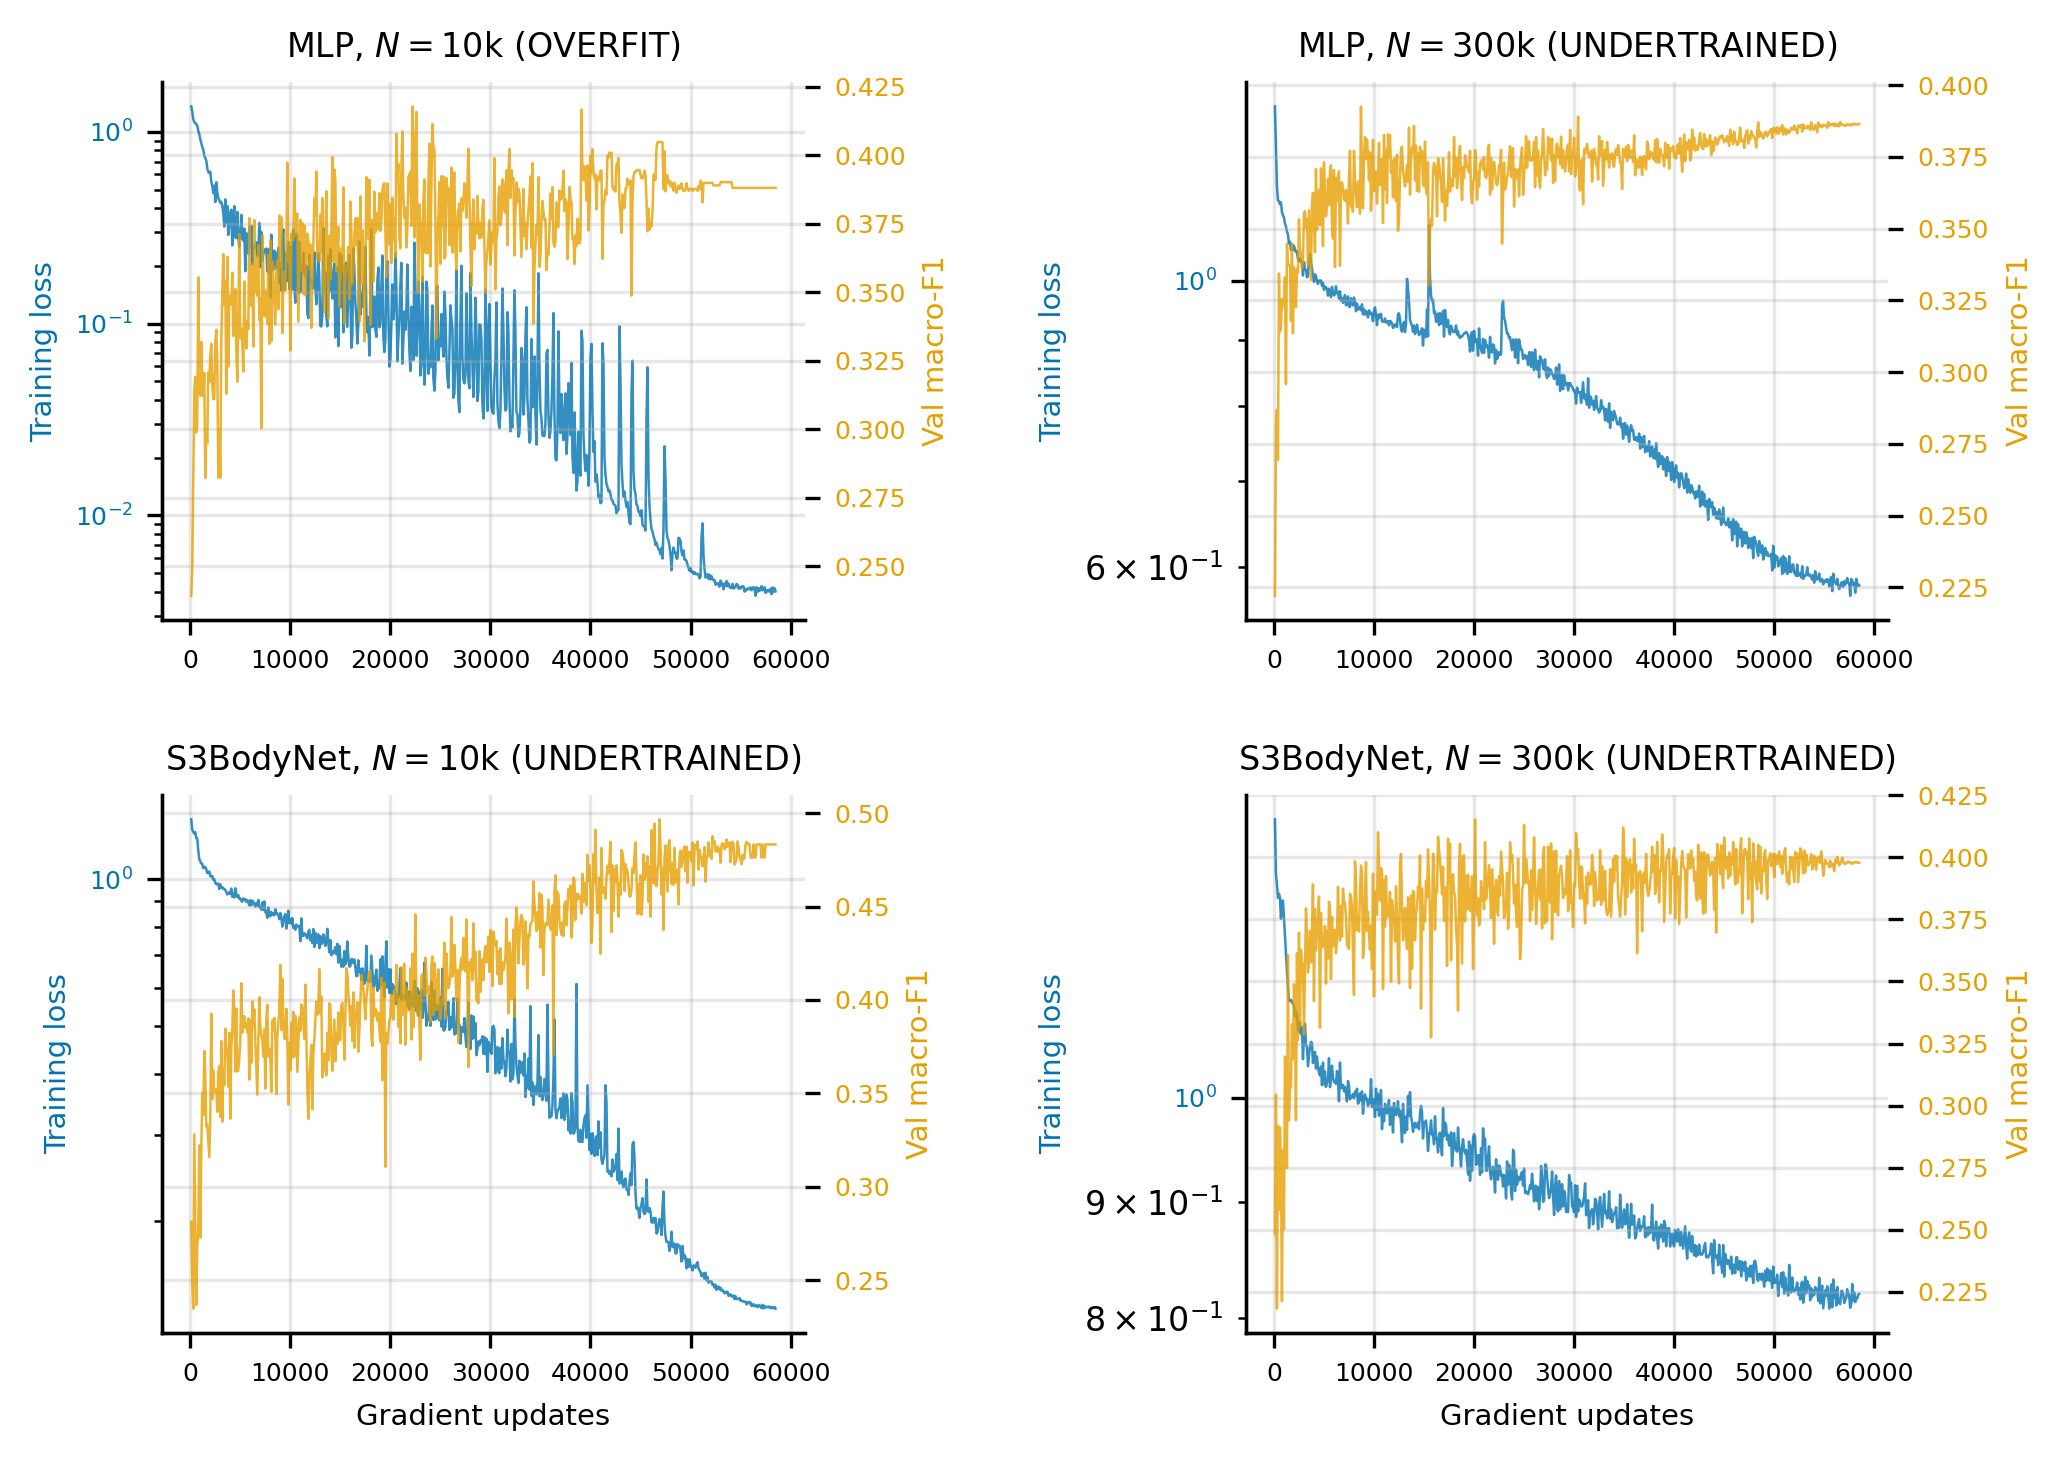
\includegraphics[width=\linewidth]{F4_diagnostic_curves.png}
  \caption{Training diagnostics for four representative cells from the matched-compute protocol. Blue: training loss (log scale). Orange: validation macro-F1. At $N = 10$k, the MLP overfits (training loss near zero, validation F1 declines from peak). At $N = 300$k, both architectures are undertrained (training loss still falling at budget end). This differential convergence biases the measured slope toward zero.}
  \label{fig:diagnostic}
\end{figure}

Figure~\ref{fig:diagnostic} reveals the mechanism. At $N = 10$k, the MLP's training loss reaches $0.005$ (near zero) while validation F1 peaks at $0.418$ and declines to $0.388$: textbook overfitting on a memorized training set. At $N = 300$k, the MLP's training loss is still $0.58$ at budget end (started at $1.12$), with validation F1 still trending upward: the model has not converged. S3BodyNet shows the same pattern more severely, as it converges slower than the MLP on zero-momentum inputs where 5 of 8 per-body features are identically zero.

The opposing biases, overfitting at small $N$ and undertraining at large $N$, inflate test error at both ends of the sample-size range, producing near-zero slopes. The flat slopes are an artifact of differential convergence, not evidence against the GOY bound.

\subsection{Interpretation}

Neither result alone settles the question. The architecture-specific result is consistent with the GOY prediction but confounds architecture with training schedule. The matched-compute result does not exhibit the predicted scaling but did not achieve equivalent convergence across cells. Whether classifier scaling matches the GOY bound under a protocol that achieves convergence parity across architectures and dataset sizes remains an open question. A future test would need to equalize convergence (for instance, via a train-to-plateau criterion) rather than equalize compute.

% ============================================================================
\section{ML-Guided Periodic Orbit Discovery}

Periodic orbits are the dynamical skeleton of chaotic systems: they organize the fractal basin structure, with basin boundaries coinciding with the stable manifolds of unstable periodic orbits. We exploit this connection to turn our trained basin classifier into a tool for discovering periodic orbits.

\textbf{Method.}\quad We identify basin-boundary candidates via $k$-nearest-neighbor label disagreement on the classified dataset: points whose neighbors have mixed predicted outcomes lie near basin boundaries, and therefore near periodic orbits. For each candidate, we integrate from rest and track the shape-sphere trajectory, searching for moments when the system returns close to its starting shape. The best candidates are refined using gradient-based optimization through the integrator via JAX automatic differentiation.

\textbf{Results.}\quad We searched 5{,}000 boundary candidates in 88 seconds on an NVIDIA A100 GPU. Of these, 543 exhibited near-returns (return distance $<0.05$ on the shape sphere), an 11\% hit rate compared to near-zero for random sampling. After refinement, four candidates were classified as near-periodic (return distance $<0.01$):

\begin{table}[t]
\centering
\caption{Near-periodic orbits discovered via ML-guided boundary search. Return distance is the great-circle distance on the shape sphere between the starting and returning configurations.}
\label{tab:orbits}
\begin{tabular}{lccc}
\toprule
Orbit & Period $T$ & Return distance & Energy \\
\midrule
\#1 & 11.709 & 0.0043 & $-3.404$ \\
\#6 & 0.303 & 0.0044 & $-3.535$ \\
\#7 & 0.303 & 0.0045 & $-3.535$ \\
\#9 & 0.303 & 0.0064 & $-3.000$ \\
\bottomrule
\end{tabular}
\end{table}

Orbits \#6 and \#7 form an $S_3$-symmetric pair (identical energy and period, related by body relabeling). Orbit \#9 has a distinct energy and constitutes a separate orbit family. Figure~\ref{fig:orbits} shows two representative trajectories.

\begin{figure}[t]
  \centering
  \begin{minipage}[t]{0.48\linewidth}
    \centering
    
\includegraphics[width=\linewidth]{periodic_orbit_1.png}
    \captionof{figure}{Orbit \#1 ($T = 11.7$): a complex multi-loop trajectory. Circles mark starting positions; squares mark positions after one near-period.}
    \label{fig:orbit1}
  \end{minipage}\hfill
  \begin{minipage}[t]{0.48\linewidth}
    \centering
    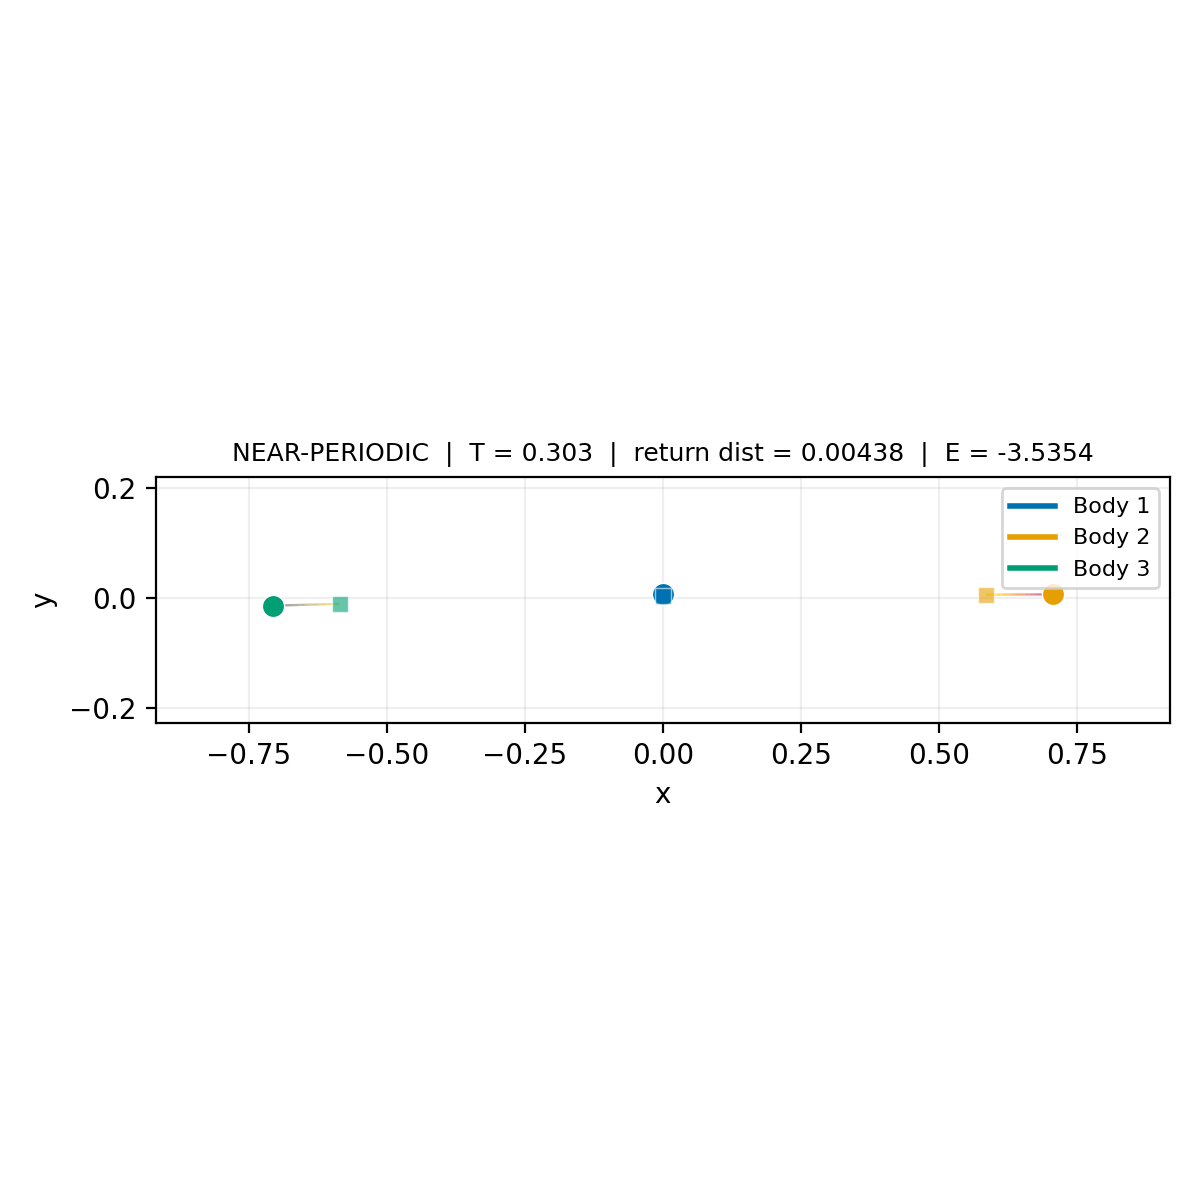
\includegraphics[width=\linewidth]{periodic_orbit_6.png}
    \captionof{figure}{Orbit \#6 ($T = 0.3$): a short-period collinear brake orbit. The nearly collinear bodies oscillate and return close to their starting configuration.}
    \label{fig:orbit6}
  \end{minipage}
\end{figure}

\textbf{Novelty.}\quad Previous approaches to three-body periodic orbit discovery use grid search \citep{Suvakov2013}, supercomputer-scale numerical simulation \citep{LiLiao2017}, or neural networks to interpolate known orbits to new parameters. Our method is the first, to our knowledge, to use a trained basin classifier's decision boundaries as a sampling prior for orbit discovery in the general three-body problem. The classifier was never trained on periodic orbits; it learned basin boundaries for escape prediction, and those boundaries coincide with the unstable manifolds of periodic orbits by the structure of chaotic scattering.

% ============================================================================
\section{Discussion}

\textbf{Active learning and dimensionality.}\quad The failure of boundary-targeted active learning in 6D is not specific to the three-body problem. Any system whose basin boundary has $D_u$ close to $d$ will exhibit spatially uniform uncertainty, rendering targeted acquisition no better than random sampling. This suggests that active-learning practitioners working on high-dimensional chaotic systems should check $D_u$ before investing in boundary-detection heuristics.

\textbf{Scaling laws and methodology.}\quad The GOY bound is a statement about asymptotic scaling under optimal classifiers. Testing it with finite neural networks introduces confounds, training dynamics, learning-rate schedules, and convergence rates, that are not part of the theoretical framework. Our results illustrate that bounds from nonlinear dynamics are not trivially testable under standard ML evaluation methodology.

\textbf{Limitations.}\quad This study is restricted to equal-mass bodies in the plane. Unequal masses, post-Newtonian corrections, and energy-conditioned sampling are not covered. The Yoshida-6 integrator without explicit close-encounter regularization is inadequate for hierarchical triples; we address this via conservative close-encounter exclusion (Appendix~\ref{app:integrator}). The 2D at-rest slice is a measure-zero subset of the full phase space, though it captures the essential fractal structure.

\textbf{Future directions.}\quad Natural extensions include transfer to other chaotic-scattering benchmarks (H\'enon-Heiles), comparison with graph neural networks and equivariant transformer architectures, and a matched-protocol test with convergence-based stopping.

% ============================================================================
\section{Conclusion}

We release a benchmark for fractal-basin classification on the planar three-body problem, with $10^6$ labeled trajectories in 2D and 6D, Wada topology characterization, and measured uncertainty exponents. Active learning helps in 2D ($+3.7\%$) but fails in 6D ($-0.7\%$), explained by the uncertainty dimension $D_u = 5.86$. Whether classifier error scaling matches the four-decade-old GOY prediction under properly matched training is an open problem; our pre-registered test and its diagnostic provide a concrete starting point. Finally, we demonstrate that the trained basin classifier can guide the discovery of periodic orbits: searching near the classifier's decision boundaries yields a 11\% hit rate, producing four near-periodic orbits in 88 seconds on a single GPU. Dataset and code are publicly available.

% ============================================================================
\bibliographystyle{plainnat}
\bibliography{refs}

% ============================================================================
\clearpage
\appendix

\section{Integrator Validation}\label{app:integrator}

We use a 6th-order Yoshida symplectic integrator \citep{Yoshida1990} with adaptive timestep. We validate on the Chenciner-Montgomery figure-eight orbit \citep{ChencinerMontgomery2000} (Figure~\ref{fig:figure_eight}), achieving relative energy conservation below $10^{-12}$ over 100 orbital periods (Figure~\ref{fig:energy}). For general initial conditions, energy is conserved to $10^{-8}$ or better over the integration window.

\begin{figure}[h]
  \centering
  \begin{minipage}[t]{0.38\linewidth}
    \centering
    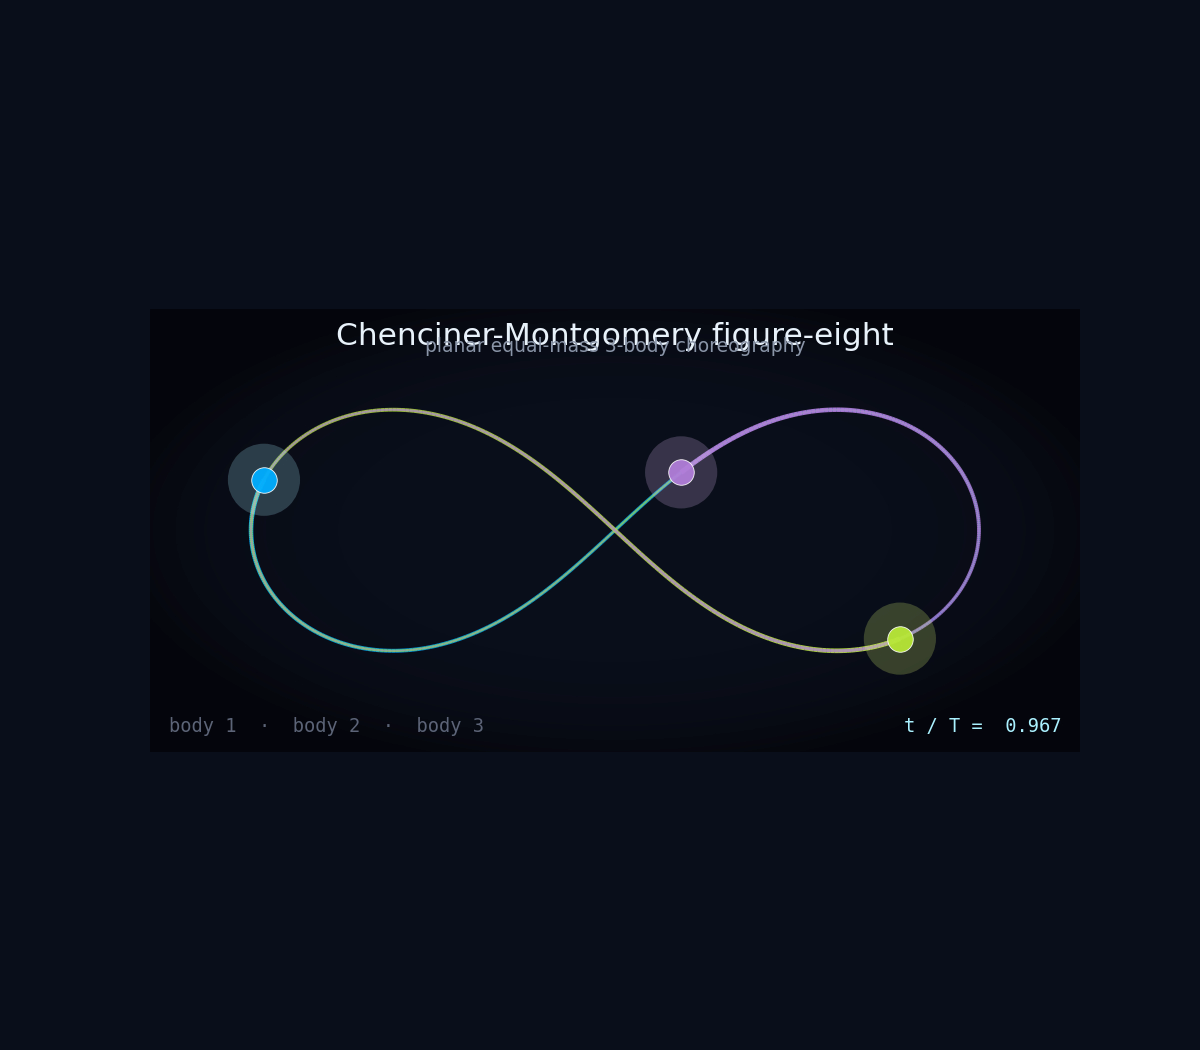
\includegraphics[width=\linewidth]{figure_eight.png}
    \captionof{figure}{The Chenciner-Montgomery figure-eight periodic orbit used for integrator validation. Three equal-mass bodies chase each other along a single figure-eight trajectory.}
    \label{fig:figure_eight}
  \end{minipage}\hfill
  \begin{minipage}[t]{0.58\linewidth}
    \centering
    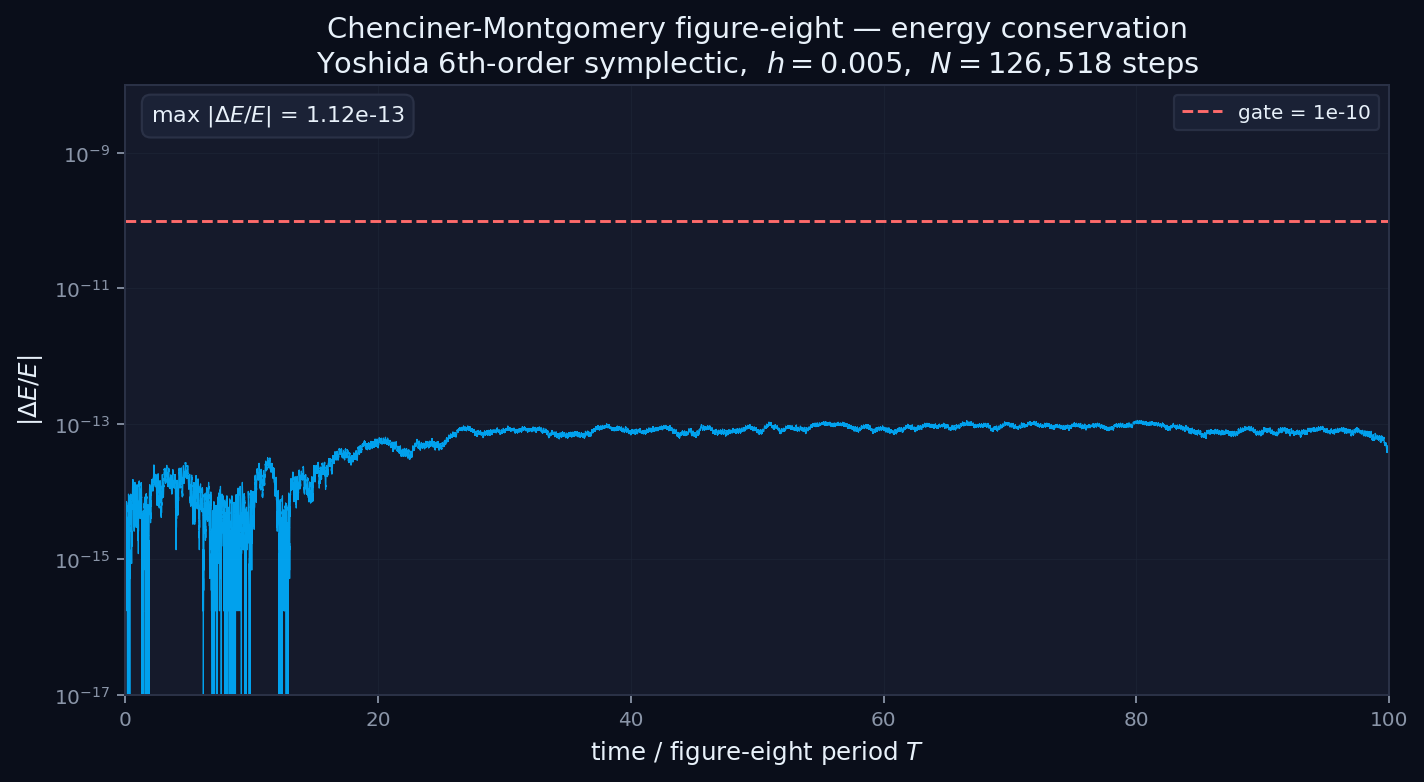
\includegraphics[width=\linewidth]{figure_eight_energy.png}
    \captionof{figure}{Relative energy error $|\Delta E / E|$ over 100 figure-eight orbital periods. The Yoshida 6th-order symplectic integrator maintains energy conservation below $10^{-12}$ throughout, with no secular drift.}
    \label{fig:energy}
  \end{minipage}
\end{figure}

Trajectories approaching binary collision ($r_{\min} < 0.01$) experience large force gradients that degrade integration accuracy. Rather than implement explicit regularization, we exclude these trajectories, removing 9.1\% of the 2D sample and 3.4\% of the 6D sample. This is a conservative choice: excluded trajectories are disproportionately concentrated near the basin boundaries (collision singularities lie on the boundary), so their removal slightly biases the measured uncertainty exponent downward.

Integration time-cutoff sensitivity is shown in Figure~\ref{fig:timecutoff}: the bound fraction is stable across an order of magnitude in $t_{\max}$, confirming that the chosen cutoff does not materially affect the class balance.

\begin{figure}[h]
  \centering
  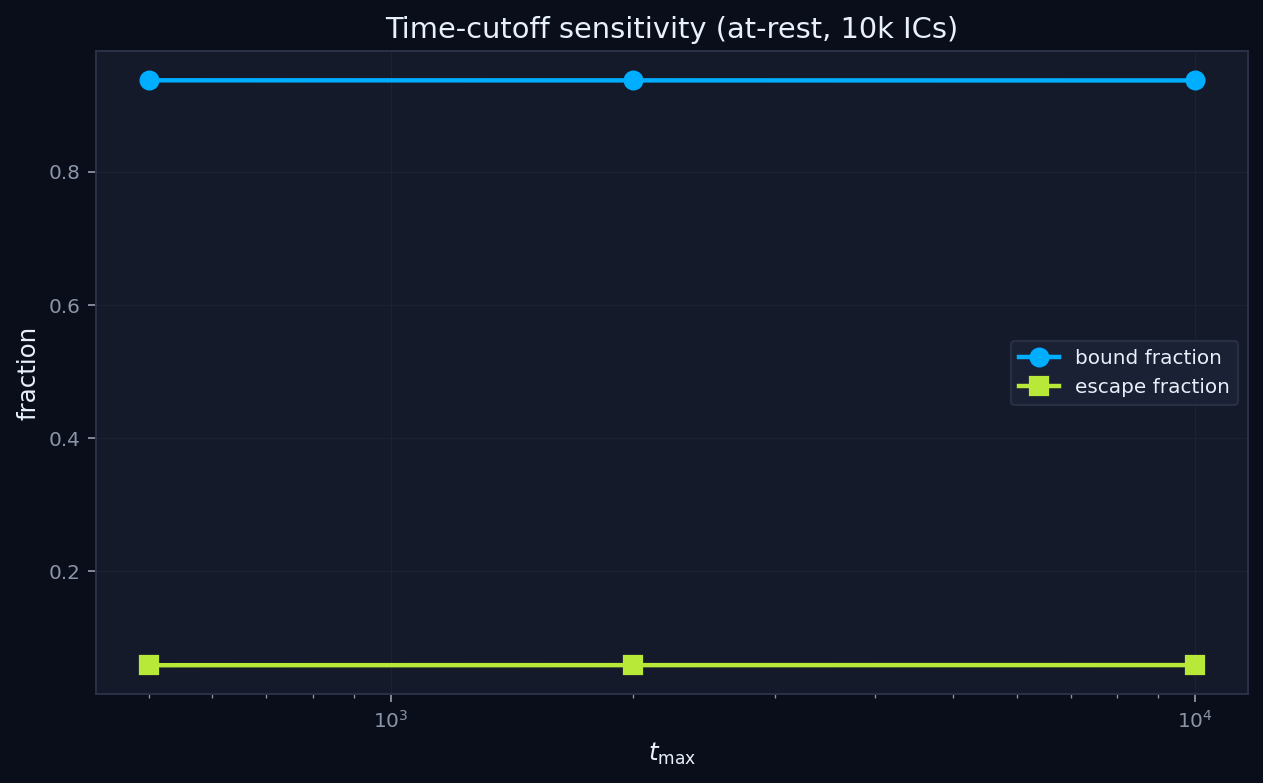
\includegraphics[width=0.6\linewidth]{time_cutoff.png}
  \caption{Bound and escape fractions as a function of the integration time cutoff $t_{\max}$, for a subsample of $10^4$ initial conditions. Both fractions are stable, indicating the classification is insensitive to the precise cutoff value.}
  \label{fig:timecutoff}
\end{figure}

\section{Uncertainty Exponent Measurement}\label{app:alpha}

\begin{figure}[h]
  \centering
  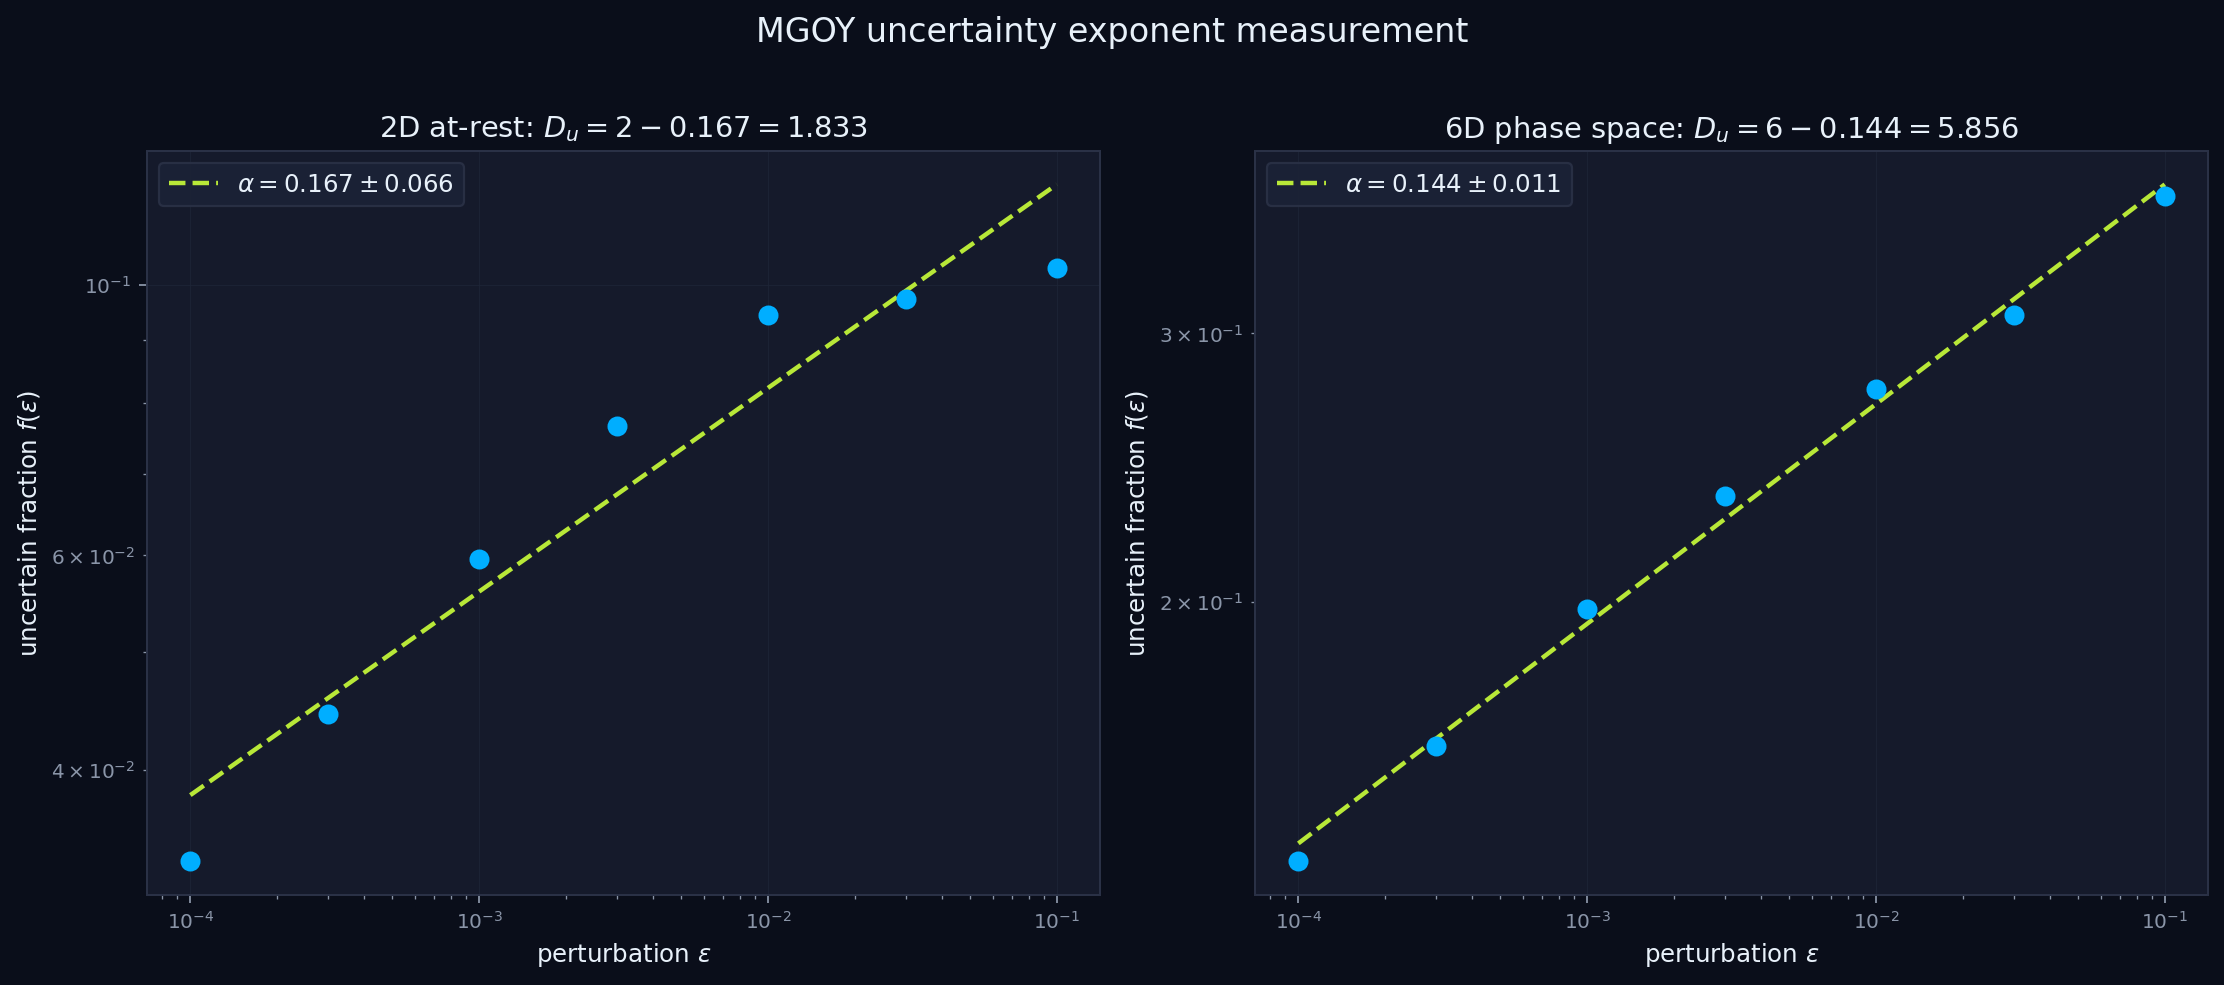
\includegraphics[width=0.85\linewidth]{uncertainty_fit.png}
  \caption{MGOY uncertainty exponent measurement. Left: 2D at-rest ($\alpha = 0.259 \pm 0.019$, $D_u = 1.74$). Right: 6D phase space ($\alpha = 0.145 \pm 0.004$, $D_u = 5.86$). Log-log plots of the uncertain fraction $f(\varepsilon)$ versus perturbation scale $\varepsilon$, with power-law fits. Both show $R^2 > 0.99$.}
  \label{fig:alpha}
\end{figure}

The MGOY algorithm \citep{MGOY1985} measures $\alpha$ by computing the fraction of initial-condition pairs separated by $\varepsilon$ that land in different basins. We use $10^5$ pairs per $\varepsilon$ value across two decades of perturbation scales. Figure~\ref{fig:alpha} shows the measurements for both 2D and 6D.

For 6D, a sliding-window analysis of local $\alpha$ across four decades of $\varepsilon$ shows variation of only 0.022, ruling out multi-fractal behavior. The boundary is uniformly fractal at all tested scales.

\section{Wada Basin Test and Basin Entropy}\label{app:wada}

\begin{figure}[h]
  \centering
  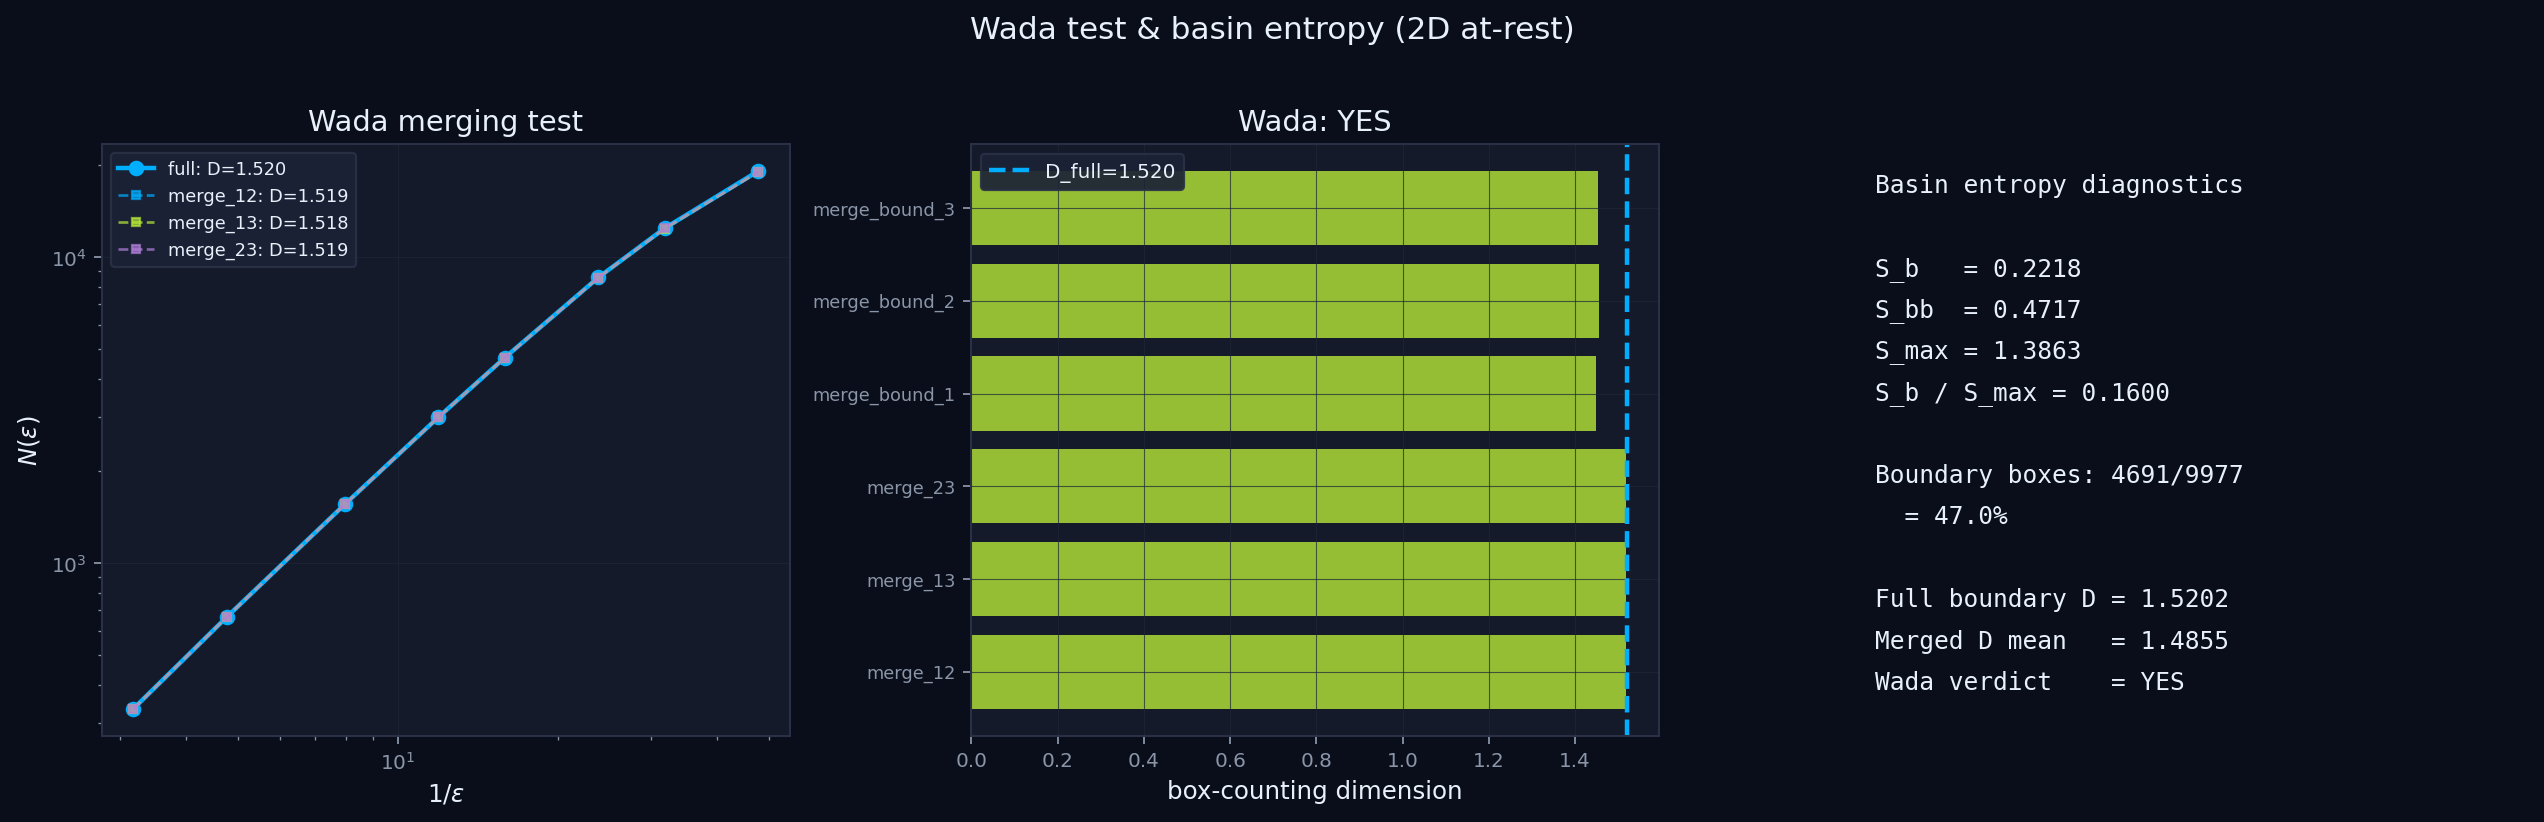
\includegraphics[width=0.85\linewidth]{wada_basin_entropy.png}
  \caption{Left: Wada merging test. The boundary fractal dimension is measured after iteratively merging basin pairs. All merged dimensions converge to the same value, confirming the Wada property. Right: Box-counting dimension distribution across grid resolutions, with basin entropy diagnostics ($S_b = 0.222$, $S_{bb} = 0.472$, Wada: YES).}
  \label{fig:wada}
\end{figure}

The merging test \citep{Daza2018} iteratively merges pairs of basin classes and checks whether the boundary fractal dimension changes. If the basin is Wada, every boundary point borders all basins, so merging any two basins leaves the boundary dimension unchanged. Figure~\ref{fig:wada} confirms this for the 2D at-rest dataset: the full boundary dimension $D = 1.52$ is preserved across all pairwise merges. Basin entropy diagnostics \citep{Daza2016} yield $S_b = 0.222$ and $S_{bb} = 0.472$, with 47\% of grid boxes lying on the boundary.

\section{Architecture Details}\label{app:arch}

\textbf{MLP.}\quad 6-layer feed-forward network, 384 hidden units per layer, GELU activation, 5 output units (4 class logits + 1 regression head for log escape time). Input: 3D shape-sphere coordinates $(n_1, n_2, n_3)$. Trained with AdamW, class-weighted cross-entropy, cosine learning-rate schedule.

\textbf{S3BodyNet.}\quad Permutation-equivariant architecture. Per-body features (8 per body: distances to the other two bodies, pairwise distance products, kinetic energies, center-of-mass distance, radial velocity, angular momentum) are concatenated with global invariants (total energy, total angular momentum, symmetric distance polynomials). A shared 4-layer MLP (256 hidden, 128 output) processes each body's features. The pooled representation produces the bound logit and regression head; per-body representations produce escape logits. Weight sharing enforces $S_3$ equivariance by construction.

Figure~\ref{fig:configs} illustrates the physical configurations corresponding to sampled shape-sphere points, showing the variety of triangle geometries encoded by the benchmark.

\begin{figure}[h]
  \centering
  
\includegraphics[width=0.75\linewidth]{shape_sphere_configs.png}
  \caption{Physical three-body configurations corresponding to sampled points on the shape sphere. Each panel shows the triangle formed by three equal-mass bodies at a given $(n_1, n_2, n_3)$ coordinate. The diversity of configurations, from near-collinear to near-equilateral, illustrates the range of initial conditions in the benchmark.}
  \label{fig:configs}
\end{figure}

\section{Matched-Compute Protocol}\label{app:protocol}

The full pre-registered protocol: AdamW with $\beta_1 = 0.9$, $\beta_2 = 0.999$, $\varepsilon = 10^{-8}$, weight decay $10^{-4}$. Batch size 1024. Linear warmup from 0 to peak learning rate over 500 steps, then cosine decay to zero over the remaining budget. Total gradient updates: $\lfloor 200 \times 300{,}000 / 1024 \rfloor = 58{,}594$. Peak learning rate tuned once per architecture on a 20\% held-out slice of the $N = 10$k training set over a 60-epoch trial: both architectures selected $3 \times 10^{-3}$. Five seeds $\{0, 1, 2, 3, 4\}$. No early stopping. Test metric: $1 - \text{macro-F1}$ on a fixed $10^5$ held-out test set.

\section{Four-Way Ablation}\label{app:ablation}

\begin{figure}[h]
  \centering
  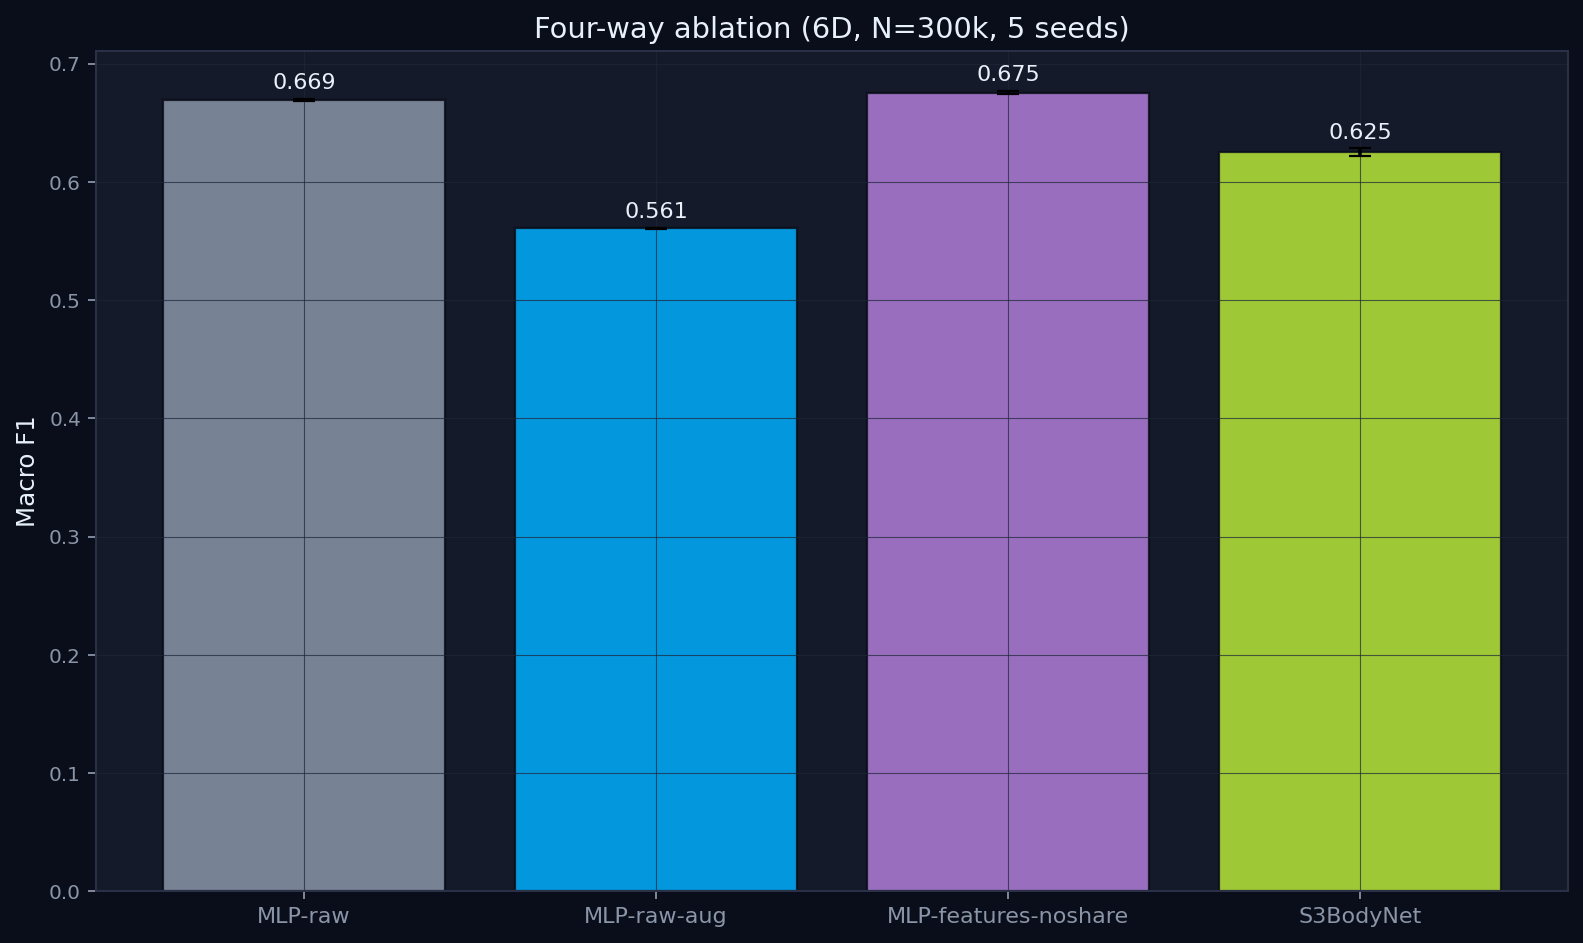
\includegraphics[width=0.65\linewidth]{ablation_n300k.png}
  \caption{Four-way architecture ablation at $N = 300$k (6D dataset, 5 seeds). MLP-features-noshare achieves the highest macro-F1 (0.675). $S_3$ data augmentation degrades performance by 10 F1 points, consistent with capacity dilution on already-symmetric data.}
  \label{fig:ablation}
\end{figure}

At $N = 10^6$ training samples (2D), the ablation results sharpen further:

\begin{table}[h]
\centering
\caption{Ablation at $N = 10^6$, 2D at-rest dataset, 5 seeds. Macro-F1 on held-out test set.}
\label{tab:ablation}
\begin{tabular}{lcc}
\toprule
Architecture & Accuracy & Macro-F1 \\
\midrule
MLP-raw (3D input) & $0.710 \pm 0.001$ & $0.699 \pm 0.001$ \\
MLP-features-noshare & $0.711 \pm 0.001$ & $0.700 \pm 0.001$ \\
S3BodyNet (equivariant) & $0.662 \pm 0.001$ & $0.646 \pm 0.001$ \\
MLP-raw + $S_3$ augmentation & $0.601 \pm 0.001$ & $0.574 \pm 0.001$ \\
\bottomrule
\end{tabular}
\end{table}

MLP-raw and MLP-features-noshare tie at $N = 10^6$: hand-crafted features provide no additional benefit at this sample size. S3BodyNet's built-in equivariance does not compensate for its slower convergence on zero-momentum inputs. Data augmentation with $S_3$ group elements actively degrades performance, consistent with a capacity-dilution effect on data that is already $S_3$-symmetric.

\section{Null and Negative Results}\label{app:null}

\textbf{6D scaling law.}\quad The GOY prediction for 6D is $-\alpha_{6D}/6 = -0.024$. The measured MLP slope in 6D is approximately $-0.054$, a factor of $2.2\times$ steeper. The $\alpha_{6D}$ measurement is clean ($R^2 = 0.999$) and the boundary is not multi-fractal (local $\alpha$ varies by only 0.022 across four decades of $\varepsilon$). The disagreement between predicted and measured slopes in 6D is unexplained.

\textbf{SIREN architecture.}\quad A SIREN network (sinusoidal activations) was tested as an alternative to the GELU-based MLP. Performance was indistinguishable from the baseline MLP at $N = 300$k and $N = 10^6$. We do not report SIREN results in the main text.

\section{Periodic Orbit Search Details}\label{app:orbits}

\textbf{Candidate selection.}\quad We compute $k$-nearest-neighbor label disagreement ($k=5$) on the first 50{,}000 points of the classified 2D at-rest dataset. Points where more than 30\% of neighbors have a different label are flagged as boundary candidates. From these, we select the 5{,}000 with highest disagreement fraction.

\textbf{Shooting protocol.}\quad Each candidate is integrated from rest (zero initial momenta) for 30{,}000 Yoshida-6 steps at $h = 0.003$ (total time $T = 90$). At each step, the configuration is projected to shape-sphere coordinates via the Hopf map. A running minimum of the great-circle distance between the current shape and the starting shape is maintained. Steps within the first 100 (to skip trivial near-returns) and steps where a pairwise distance drops below $r_{\min} = 0.01$ are excluded. Integration is vectorized across batches of 200 candidates using \texttt{jax.vmap}.

\textbf{Refinement.}\quad The top 10 candidates (by return distance) are refined via gradient descent on the return distance. The starting shape is parameterized in spherical coordinates $(\theta, \phi)$, and the gradient of the return distance with respect to $(\theta, \phi)$ is computed via JAX reverse-mode automatic differentiation through the full integration. Each candidate is refined for 300 iterations at learning rate $10^{-4}$.

\textbf{Classification.}\quad A candidate is classified as PERIODIC if the refined return distance is below 0.001 radians, NEAR-PERIODIC if below 0.01, and CANDIDATE otherwise.

\begin{figure}[h]
  \centering
  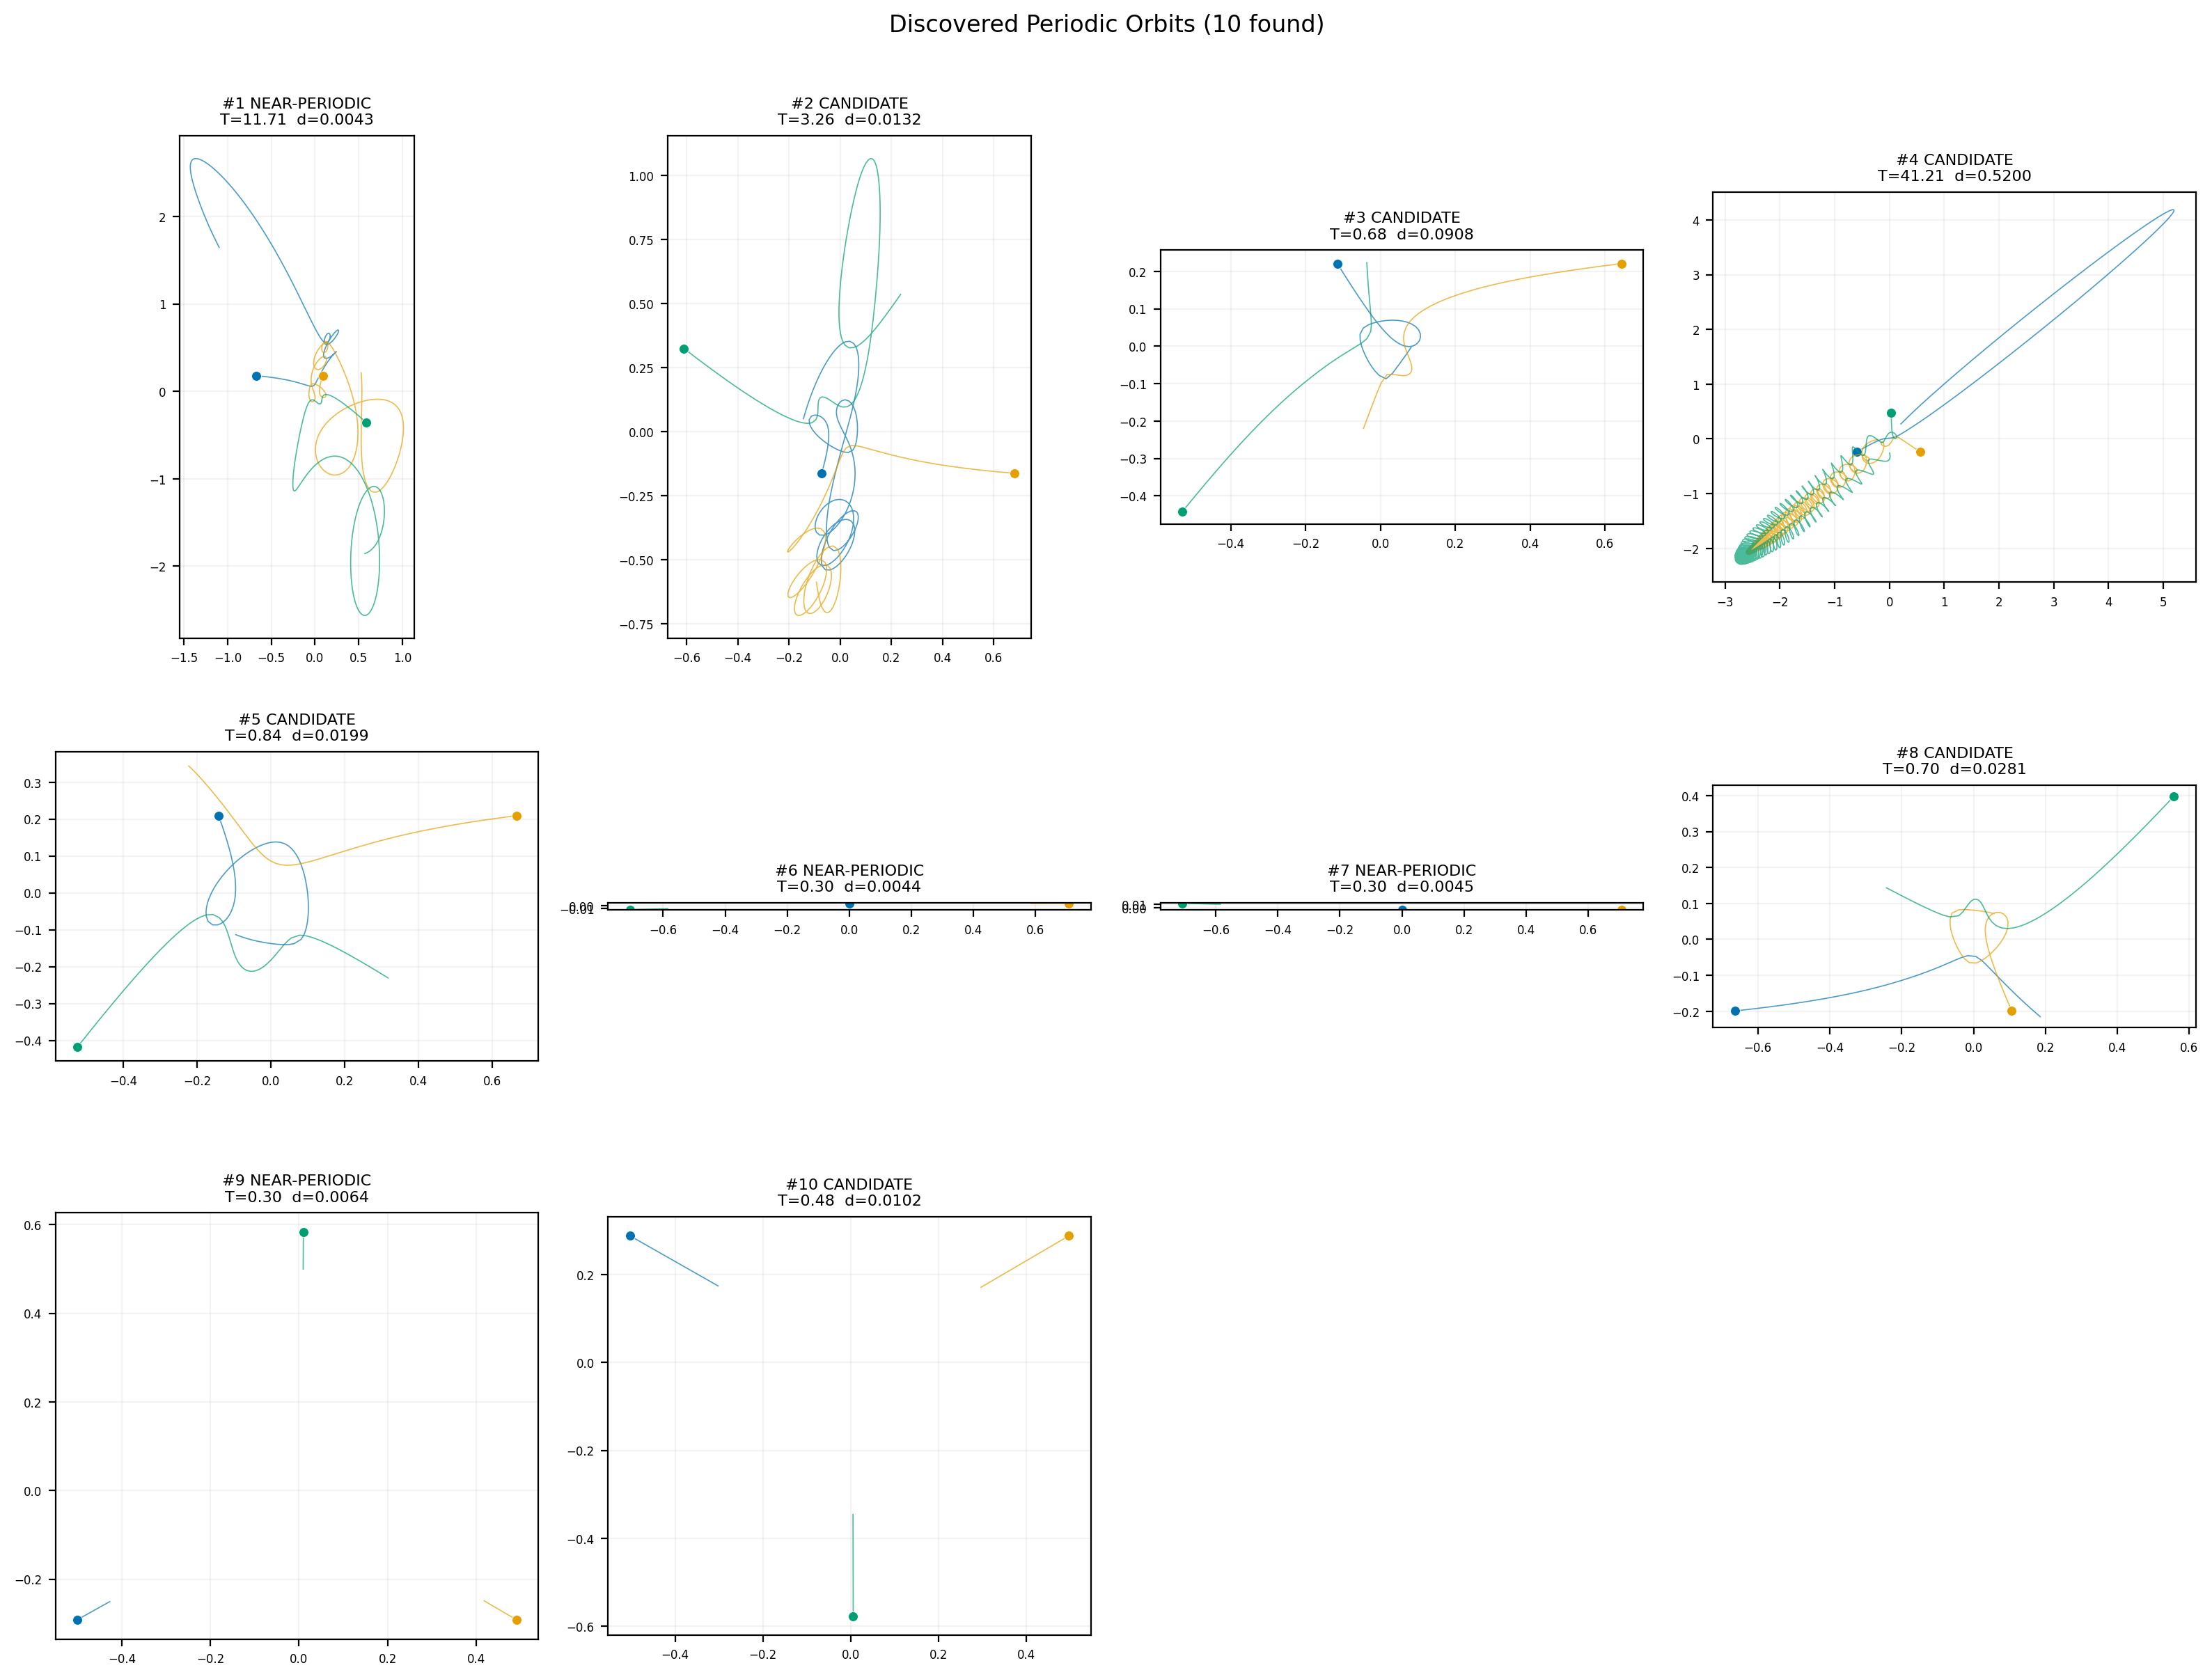
\includegraphics[width=\linewidth]{periodic_orbits_summary.png}
  \caption{All 10 orbit candidates discovered by the ML-guided search. Each panel shows the physical-space trajectories of three bodies (blue, orange, green) over one near-period. Circles mark starting positions. Four orbits (\#1, \#6, \#7, \#9) achieved near-periodic classification. Orbits \#6 and \#7 are an $S_3$-symmetric pair.}
  \label{fig:orbits_summary}
\end{figure}

\end{document}
